\newif\ifcrossling\crosslingfalse
\newif\iflong\longfalse
\newif\ifevaluation\evaluationfalse
\newif\ifconjugacy\conjugacyfalse
\newif\ifnonpar\nonparfalse
\newif\ifhighlevel\highlevelfalse
\newif\ifitmtree\itmtreetrue

\documentclass[compress]{beamer}

%\usepackage{beamerthemesplit}
\usepackage{xmpmulti}

\usepackage{graphicx,float,wrapfig, bbm}
\usepackage{amsfonts, bbold, comment}
\usepackage{mdwlist}
\usepackage{subfigure}
\usepackage{colortbl}
\usepackage{overpic}
\usepackage{algorithmic}
\usepackage{algorithm}
\usepackage{multirow}

\pgfdeclareimage[width=\paperwidth]{mybackground}{../../common/boulder.pdf}


\newcommand{\danquote}[1]{

\begin{flushright}
\begin{overpic}[width=5.5cm,tics=10]{general_figures/speech_bubble}
	\put(10,30) { \parbox{4cm}{#1 }}
\end{overpic}

\includegraphics[width=1.5cm]{general_figures/milkman_dan}
\end{flushright}
}

\newcommand{\explain}[2]{\underbrace{#2}_{\mbox{\footnotesize{#1}}}}
\newcommand{\e}[2]{\mathbb{E}_{#1}\left[ #2 \right] }
\newcommand{\ind}[1]{\mathbb{I}\left[ #1 \right] }
\newcommand{\ex}[1]{\mbox{exp}\left\{ #1\right\} }
%\newcommand{\g}{\, | \,}
\newcommand{\citename}[1]{#1 }

\newcommand{\greentext}[1]{\textcolor{caribbeangreen}{#1}}
\newcommand{\yellowtext}[1]{\textcolor{amber}{#1}}
\newcommand{\redtext}[1]{\textcolor{red}{#1}}
\newcommand{\bluetext}[1]{\textcolor{blue}{#1}}

\newcommand{\bm}[1]{\mbox{\boldmath$#1$}}
\newcommand{\Dir}{\mathrm{Dir}}
\newcommand{\Mult}{\mathrm{Mult}}
\newcommand{\g}[1]{\Gamma \left( #1 \right)}
\newcommand{\paragraph}[1]{ \vskip 1cm {\bf \large #1}}

\newcommand{\tb}[1]{\textbf{#1}}
\newcommand{\subtwo}[2]{_{#1, #2}}
\newcommand{\subthree}[3]{_{#1, #2, #3}}
\newcommand{\minussubtwo}[2]{_{-{#1, #2}}}
\newcommand{\minussubthree}[3]{_{-{#1, #2, #3}}}
\newcommand{\suptwo}[2]{^{#1, #2}}
\newcommand{\supthree}[3]{^{#1, #2, #3}}
\newcommand{\minussuptwo}[2]{^{-{#1, #2}}}
\newcommand{\minussupthree}[3]{^{-{#1, #2, #3}}}
\newcommand{\prior}[1]{\mathcal{B}#1} % to be revised

\newcommand{\gfx}[2]{
\begin{center}
	\includegraphics[width=#2\linewidth]{teaparty/figures/#1}
\end{center}
}


\usetheme[bullet=circle,                     % Use circles instead of squares for bullets.
          titleline=true,                    % Show a line below the frame title.
          showdate=true,                     % show the date on the title page
          alternativetitlepage=true,         % Use the fancy title page.
          titlepagelogo=general_figures/culogo,              % Logo for the first page.
          % Logo for the header on first page.
          headerlogo=general_figures/boulder_cs,
          ]{UCBoulder}

\usecolortheme{ucdblack}
\title[ITM]{Interactive Topic Modeling (and applications to US Tea Party)}
\author[Boyd-Graber]{Jordan Boyd-Graber (UCB)}
\date{August 2015}

\institute[Boulder] % (optional, but mostly needed)
{University of Maryland and University of Colorado Boulder}

%\AtBeginSection[] % "Beamer, do the following at the start of every section"
%{ \begin{frame} \frametitle{Outline} % make a frame titled "Outline"
%\tableofcontents[currentsection] % show TOC and highlight current section
%\end{frame} }

\begin{document}

\frame{
\titlepage
\tiny
}

\begin{frame}{Outline}

\begin{itemize}
	\item Overview of topic models 
	\item Interactive Topic Models 
	\item Using Expert-Informed Topic Models to Create Ideas Points for the Tea Party
\end{itemize}

\end{frame}



\providecommand{\graphscale}{0.6}


\newcommand{\dirfunc}[3]{ \frac{ \prod_{#1}^{#2} \g{ #3 } } { \g{ \sum_{#1}^{#2} #3 }}}
\newcommand{\dirnum}[4]{ \frac{\g{ #3 }}{#4} \prod_{#1}^{#2} }
\newcommand{\dirden}[3]{ \g{ \sum_{#1}^{#2} #3 } }

\section{Topic Model Introduction}

\begin{frame}

	\frametitle{Why topic models?}

	\begin{columns}

	\column{.3\linewidth}

	
\includegraphics[width=1\linewidth]{topic_models/newspapers}

	\column{.55\linewidth}

	\begin{itemize}
		\item Suppose you have a huge number of documents
		\item Want to know what's going on
		\item Can't read them all (e.g. every New York Times article from the 90's)
		\item Topic models offer a way to get a corpus-level view of major themes
		\pause
		\item Unsupervised
	\end{itemize}


	\end{columns}

\end{frame}

\frame{
\begin{center}
\frametitle{Conceptual Approach}
From an \textbf<1>{input corpus} and number of topics \textbf<1>{$K$} $\rightarrow$ \textbf<2>{words to topics} \\
\only<1>{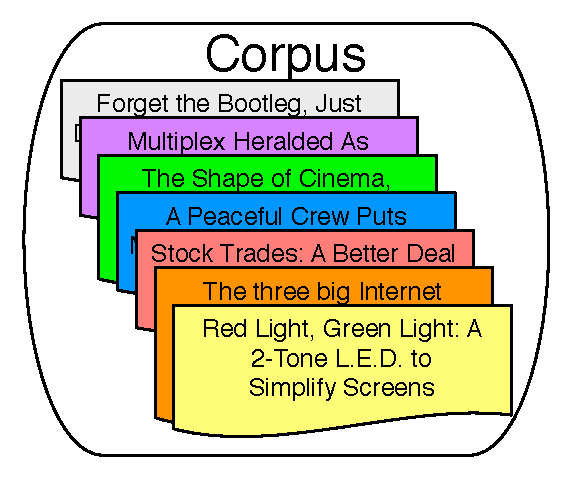
\includegraphics[width=0.6\linewidth]{reading_tea_leaves/figures/heldout_0} }
\only<2>{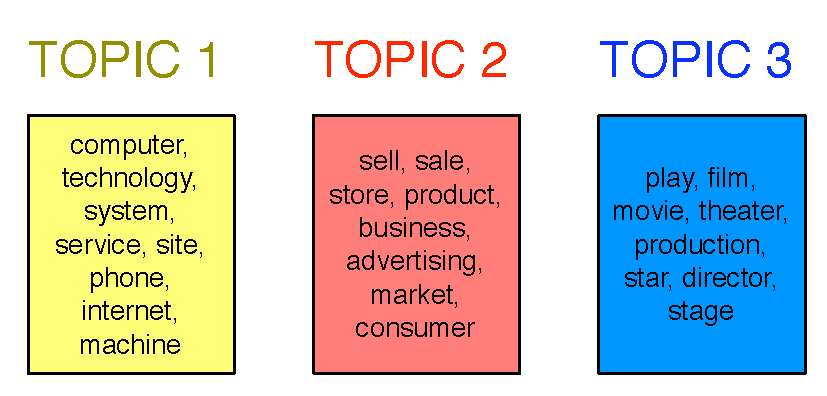
\includegraphics[width=0.9\linewidth]{reading_tea_leaves/figures/nyt_topics_wide}}
\end{center}
}

\frame{\frametitle{Conceptual Approach}

\begin{itemize}
\item For each document, what topics are expressed by that document?

\begin{center}
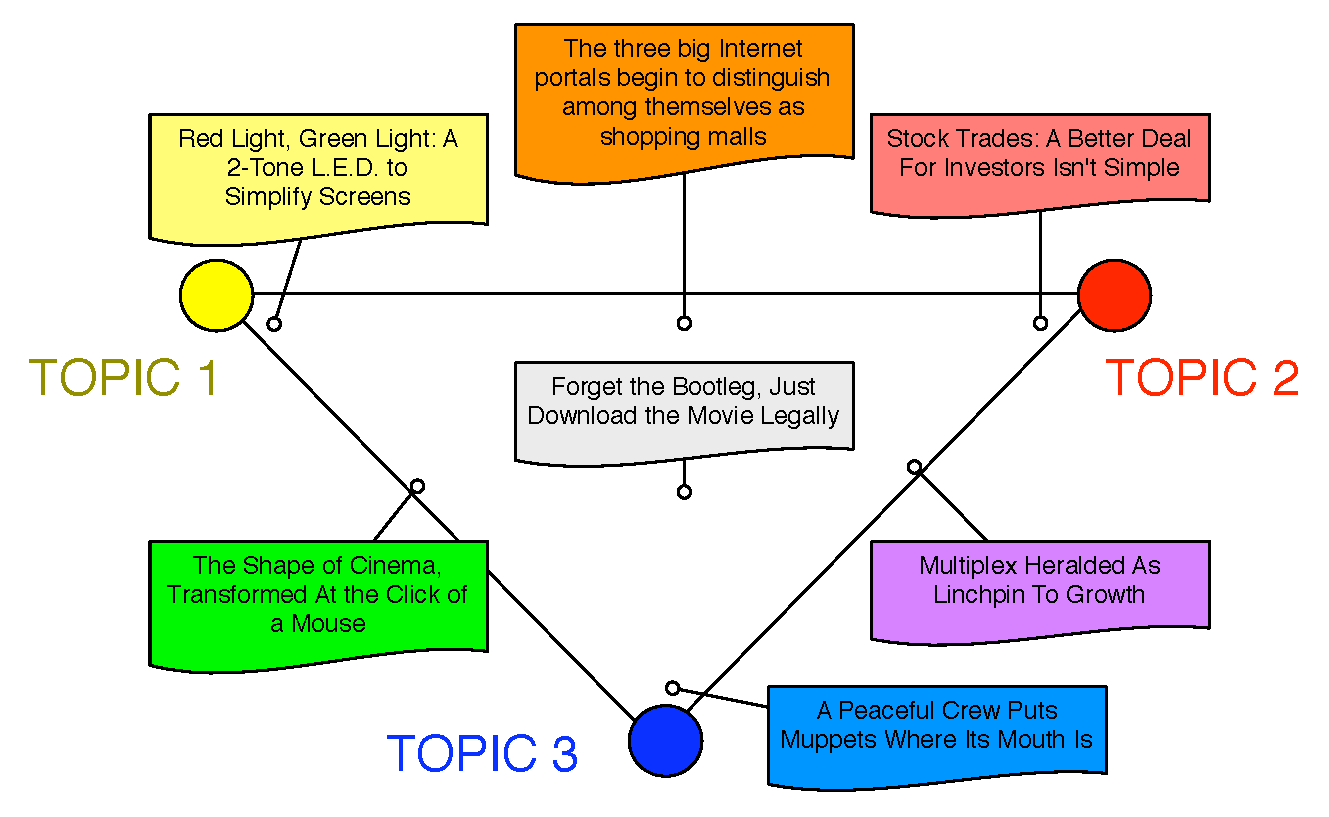
\includegraphics[width=0.9\linewidth]{topic_models/nyt_documents}
\end{center}

\end{itemize}
}

\iflong

\begin{frame}

\frametitle{Topics from \emph{Science}}

\begin{center}
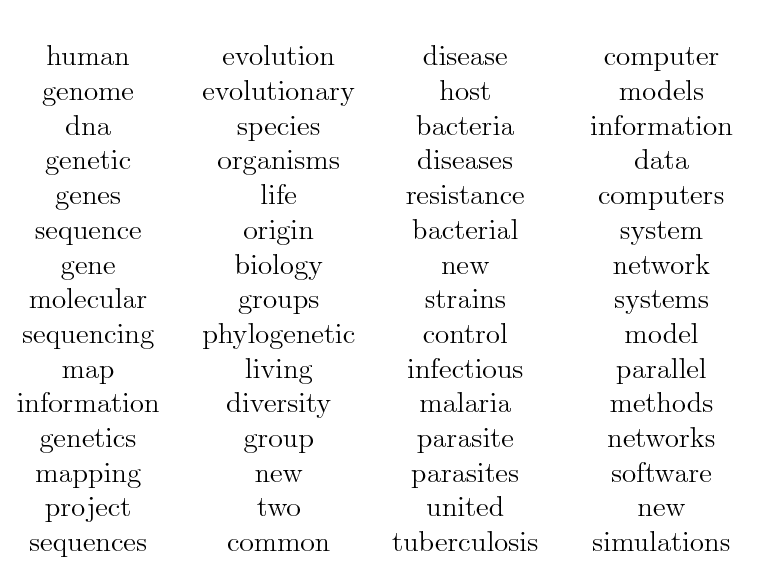
\includegraphics[width=0.8\linewidth]{topic_models/example_topics}
\end{center}

\end{frame}


\begin{frame}

\frametitle{Why should you care?}

\begin{itemize}
\item Neat way to explore / understand corpus collections
\begin{itemize}
	\item E-discovery
	\item Social media
	\item Scientific data
\end{itemize}
\item NLP Applications
\begin{itemize}
   \item POS Tagging~\cite{toutanova-08}
   \item Word Sense Disambiguation~\cite{boyd-graber-07}
   \item Word Sense Induction~\cite{brody-09}
   \item Discourse Segmentation~\cite{purver-06}
\end{itemize}
\item Psychology~\cite{griffiths-07}: word meaning, polysemy
\item Inference is (relatively) simple
\end{itemize}

\end{frame}

\frame
{
  \frametitle{Matrix Factorization Approach}

\begin{center}
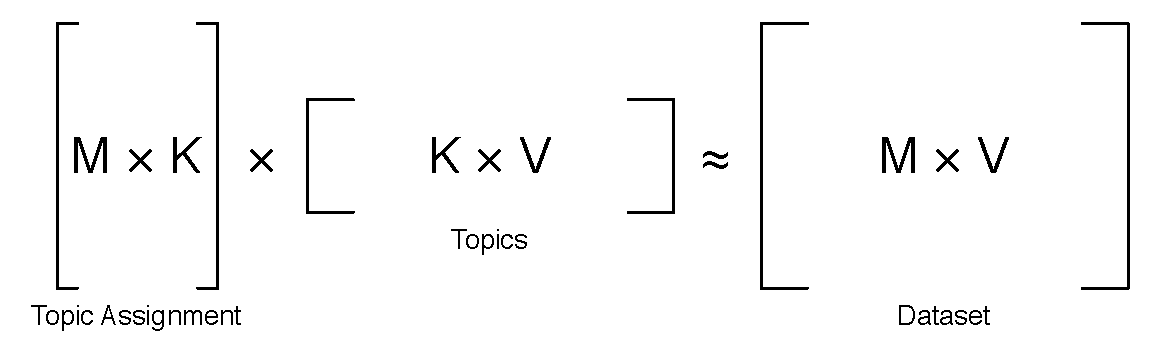
\includegraphics[width=0.9\linewidth]{topic_models/factorization.pdf}
\end{center}

\begin{columns}
\column{.5\textwidth}
\begin{block}{}
	\begin{itemize}
		\item[K] Number of topics
		\item[M] Number of documents
		\item[V] Size of vocabulary
	\end{itemize}
\end{block}
\column{.5\textwidth}
\pause
\begin{itemize}
\item If you use singular value decomposition (SVD), this technique is called latent semantic analysis.
\item Popular in information retrieval.
\end{itemize}
\end{columns}

}

\begin{frame}

\frametitle{Alternative: Generative Model}

\begin{itemize}
  \item How your data came to be
  \item Sequence of Probabilistic Steps
  \item Posterior Inference
\end{itemize}

\end{frame}

\begin{frame}
	\frametitle{Multinomial Distribution}

	\begin{itemize}
		\item Distribution over discrete outcomes
		\item Represented by non-negative vector that sums to one
		\item Picture representation
	\begin{center}
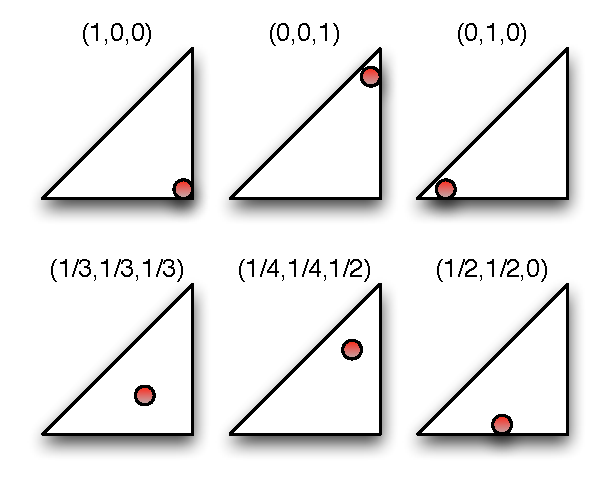
\includegraphics[width=0.4\linewidth]{topic_models/multinomial}
	\end{center}
		\pause
		\item Come from a Dirichlet distribution

	\end{itemize}


\end{frame}

\begin{frame}

\frametitle{Dirichlet Distribution}

\begin{center}
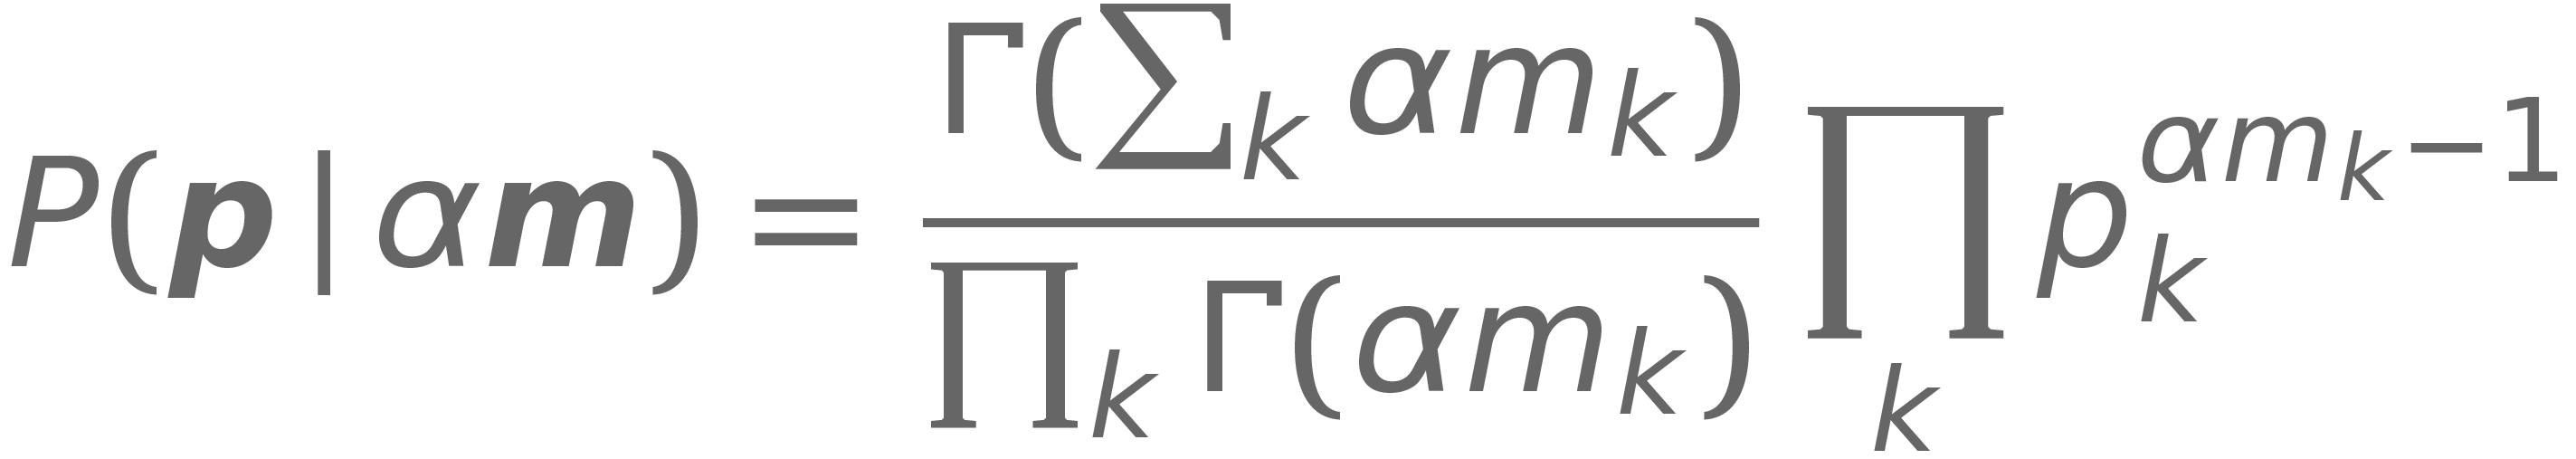
\includegraphics[width=0.4\linewidth]{topic_models/equations/dirichlet} \\ \bigskip
\pause
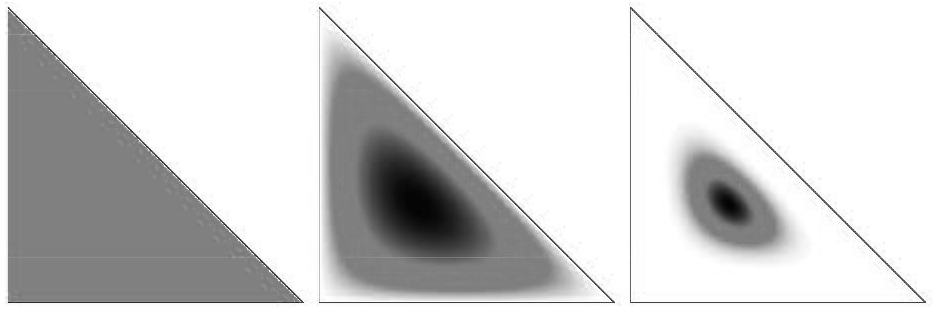
\includegraphics[width=0.6\linewidth]{topic_models/dirichlet_1} \\
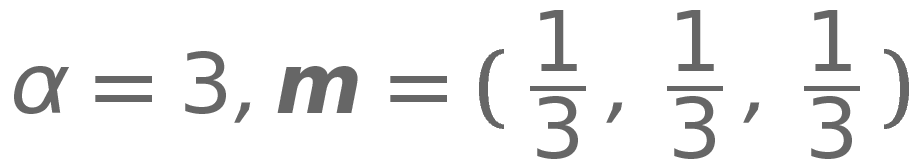
\includegraphics[width=0.2\linewidth]{topic_models/equations/dirichlet_params_1} 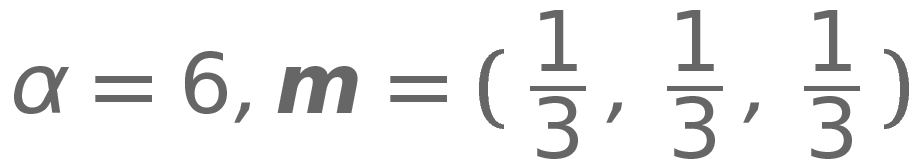
\includegraphics[width=0.2\linewidth]{topic_models/equations/dirichlet_params_2} 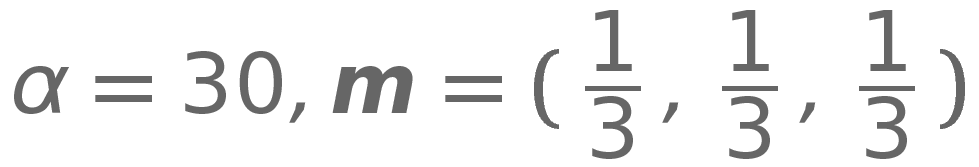
\includegraphics[width=0.2\linewidth]{topic_models/equations/dirichlet_params_3} \\
\pause
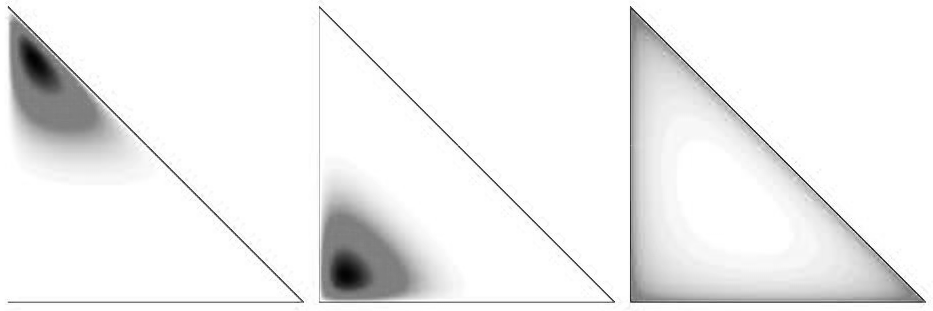
\includegraphics[width=0.6\linewidth]{topic_models/dirichlet_2} \\
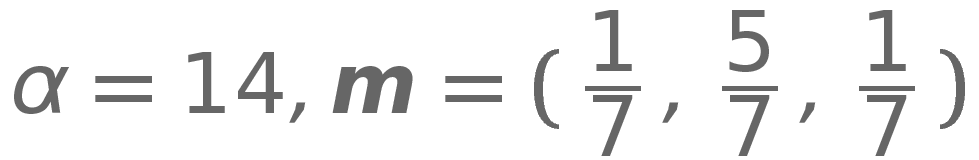
\includegraphics[width=0.2\linewidth]{topic_models/equations/dirichlet_params_4} 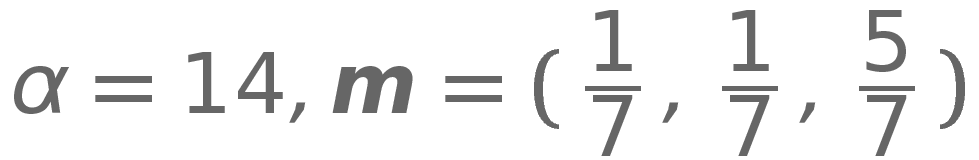
\includegraphics[width=0.2\linewidth]{topic_models/equations/dirichlet_params_5} 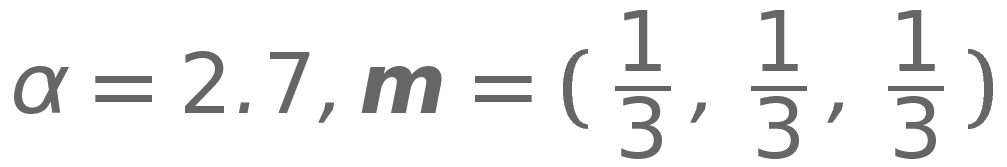
\includegraphics[width=0.2\linewidth]{topic_models/equations/dirichlet_params_6} \\
\end{center}

\end{frame}

\begin{frame}
\frametitle{Dirichlet Distribution}
\begin{center}
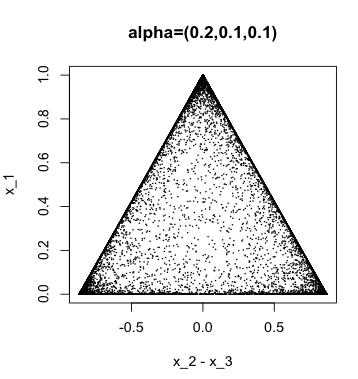
\includegraphics[width=0.5\linewidth]{topic_models/sparsity}
\end{center}
\end{frame}

\fi
\ifconjugacy

\begin{frame}
\frametitle{Dirichlet Distribution}
\begin{itemize}
  \item If ${\bm \phi} \sim \Dir(\alpha)$, ${\bm w} \sim \Mult(\phi)$, and $n_k = |\{ w_i : w_i = k\}|$ then
  \begin{align}
  	p(\phi | \alpha, {\bm w}) & \propto p({\bm w} | \phi) p(\phi | \alpha) \\
	                       & \propto  \prod_{k} \phi^{n_k} \pause  \prod_k { \phi^{\alpha_k - 1}} \\
	                       & \propto \prod_k \phi^{\alpha_k + n_k - 1}
  \end{align}
  \item Conjugacy: this {\bf posterior} has the same form as the {\bf prior}
\end{itemize}
\end{frame}

\fi

\ifhighlevel

\else

\frame
{
  \frametitle{Generative Model Approach}

\begin{center}
\only<1>{ 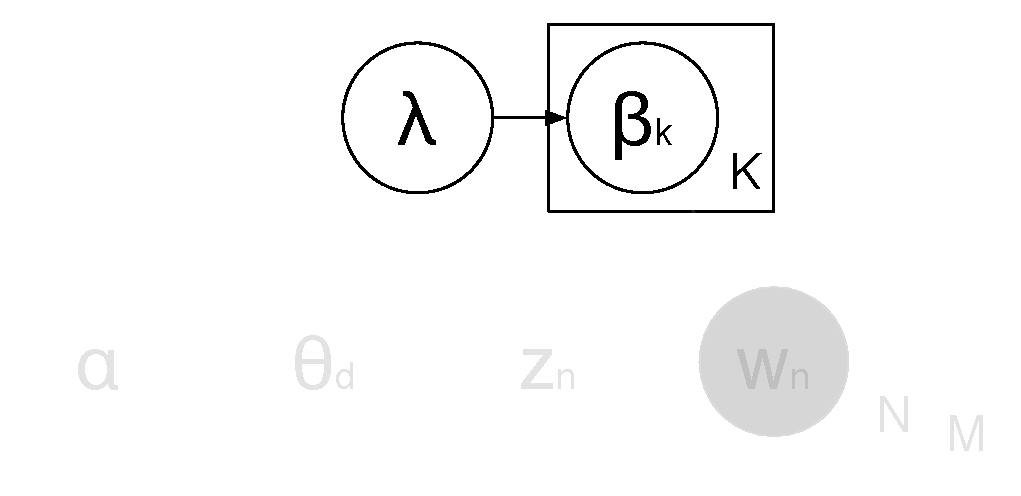
\includegraphics[scale=0.4]{topic_models/lda1.pdf} }
\only<2>{ 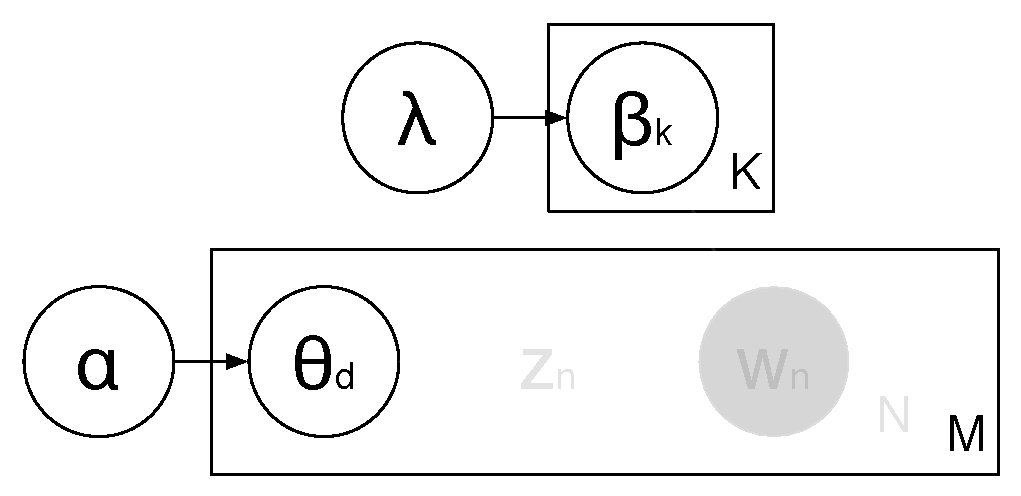
\includegraphics[scale=0.4]{topic_models/lda2.pdf} }
\only<3>{ 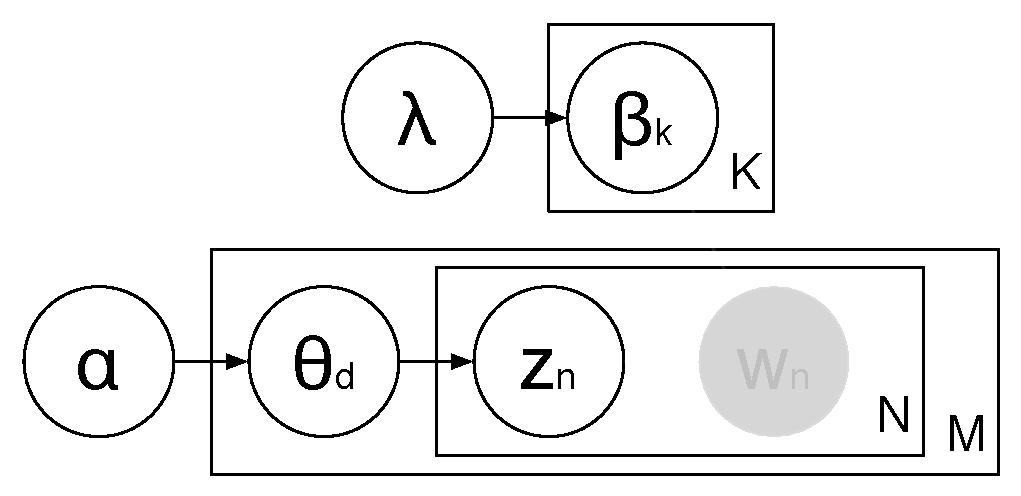
\includegraphics[scale=0.4]{topic_models/lda3.pdf} }
\only<4->{ 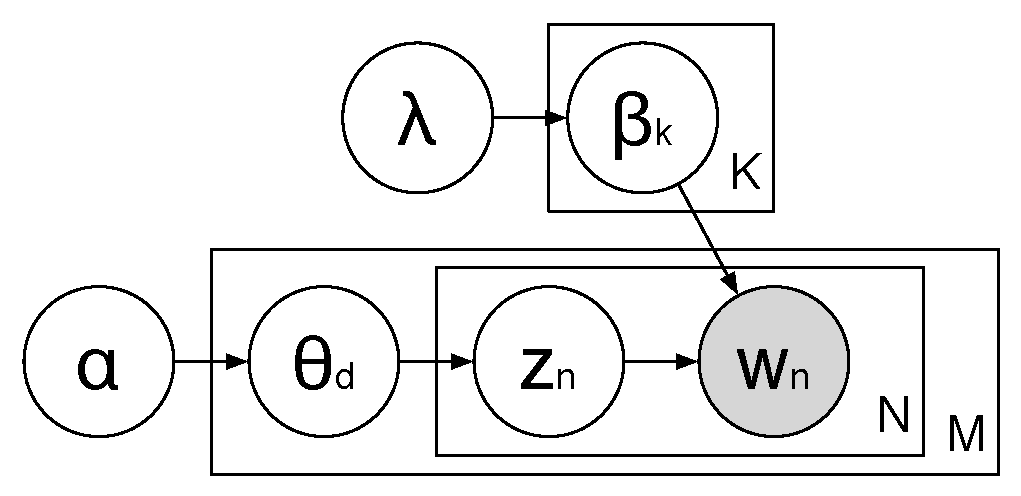
\includegraphics[scale=0.4]{topic_models/lda4.pdf} }
\end{center}

\begin{itemize}
\item<1-> For each topic $k \in \{1, \dots, K\}$, draw a multinomial distribution $\beta_k$ from a Dirichlet distribution with parameter $\lambda$
\item<2-> For each document $d \in \{1, \dots, M\}$, draw a multinomial distribution $\theta_d$ from a Dirichlet distribution with parameter $\alpha$
\item<3-> For each word position $n \in \{1, \dots, N\}$, select a hidden topic $z_n$ from the multinomial distribution parameterized by $\theta$.
\item<4-> Choose the observed word $w_n$ from the distribution $\beta_{z_n}$.
\end{itemize}

\only<5->{We use statistical inference to uncover the most likely unobserved variables given observed data.}
}

\fi

\begin{frame}
\frametitle{Topic Models: What's Important}
\begin{itemize}
\item Topic models \only<2>{(latent variables)}
\begin{itemize}
\ifhighlevel
	\item Topics to words
	\item Documents to topics
\else
	\item Topics to words---multinomial distribution
	\item Documents to topics---multinomial distribution
\fi
\end{itemize}
\item Focus in this talk: statistical methods
  \begin{itemize}
    \item Model: story of how your data came to be
    \item Latent variables: missing pieces of your story
    \item Statistical inference: filling in those missing pieces
  \end{itemize}
\item We use latent Dirichlet allocation (LDA)~\cite{blei-03}, a fully Bayesian
  version of pLSI~\cite{hofmann-99}, probabilistic version of
  LSA~\cite{landauer-97}
\end{itemize}

\end{frame}

\ifevaluation


\frame{
\frametitle{Evaluation}
\begin{center}
%\only<1>{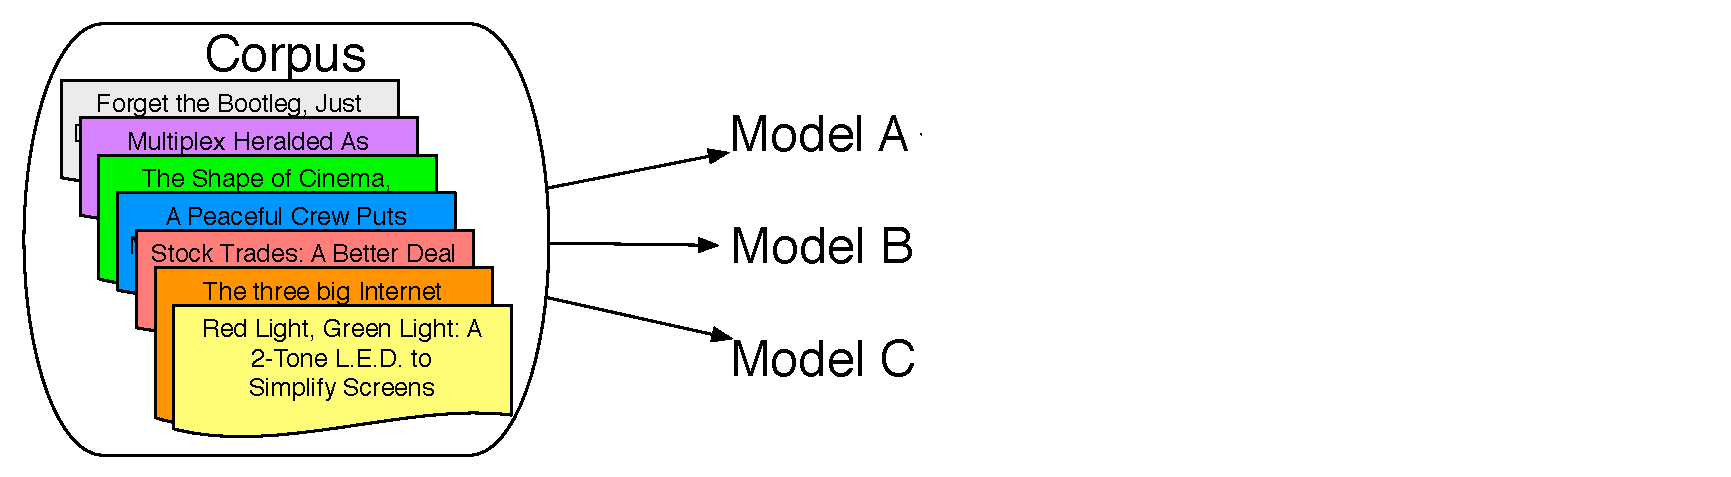
\includegraphics[width=0.9\linewidth]{reading_tea_leaves/figures/heldout_1} }
\only<1>{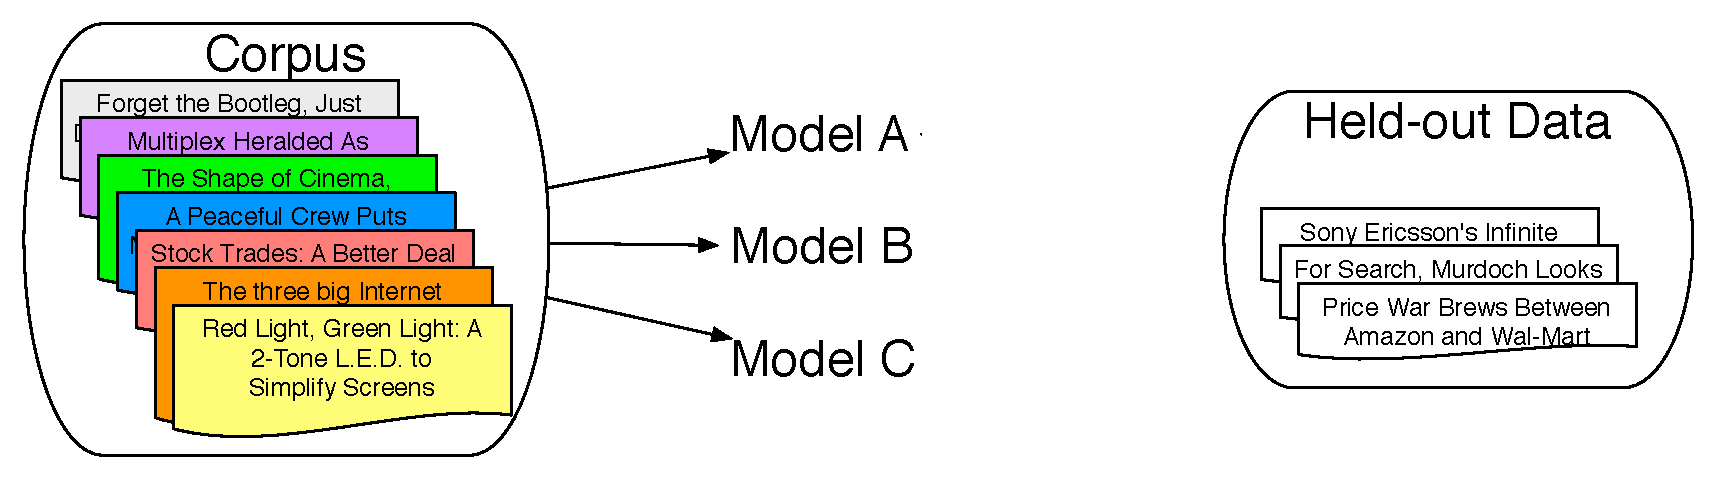
\includegraphics[width=\linewidth]{reading_tea_leaves/figures/heldout_2} }
%\only<3>{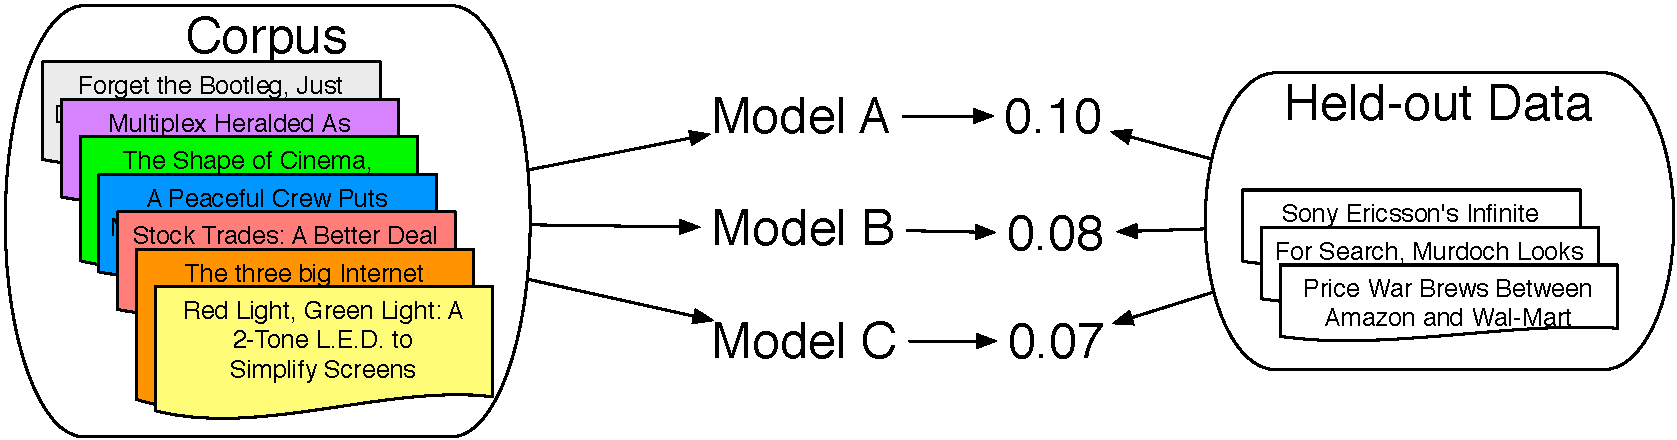
\includegraphics[width=\linewidth]{reading_tea_leaves/figures/heldout_3} }
\only<2>{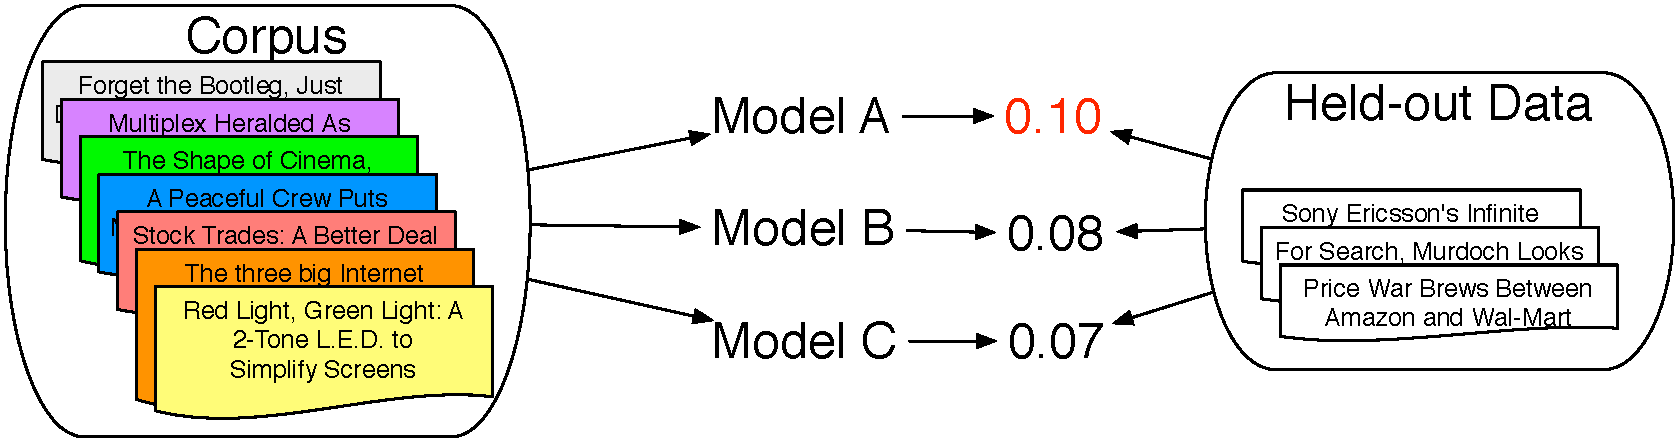
\includegraphics[width=\linewidth]{reading_tea_leaves/figures/heldout_4}  \\
	\large Measures predictive power, not what the topics are}
\end{center}

\begin{center}
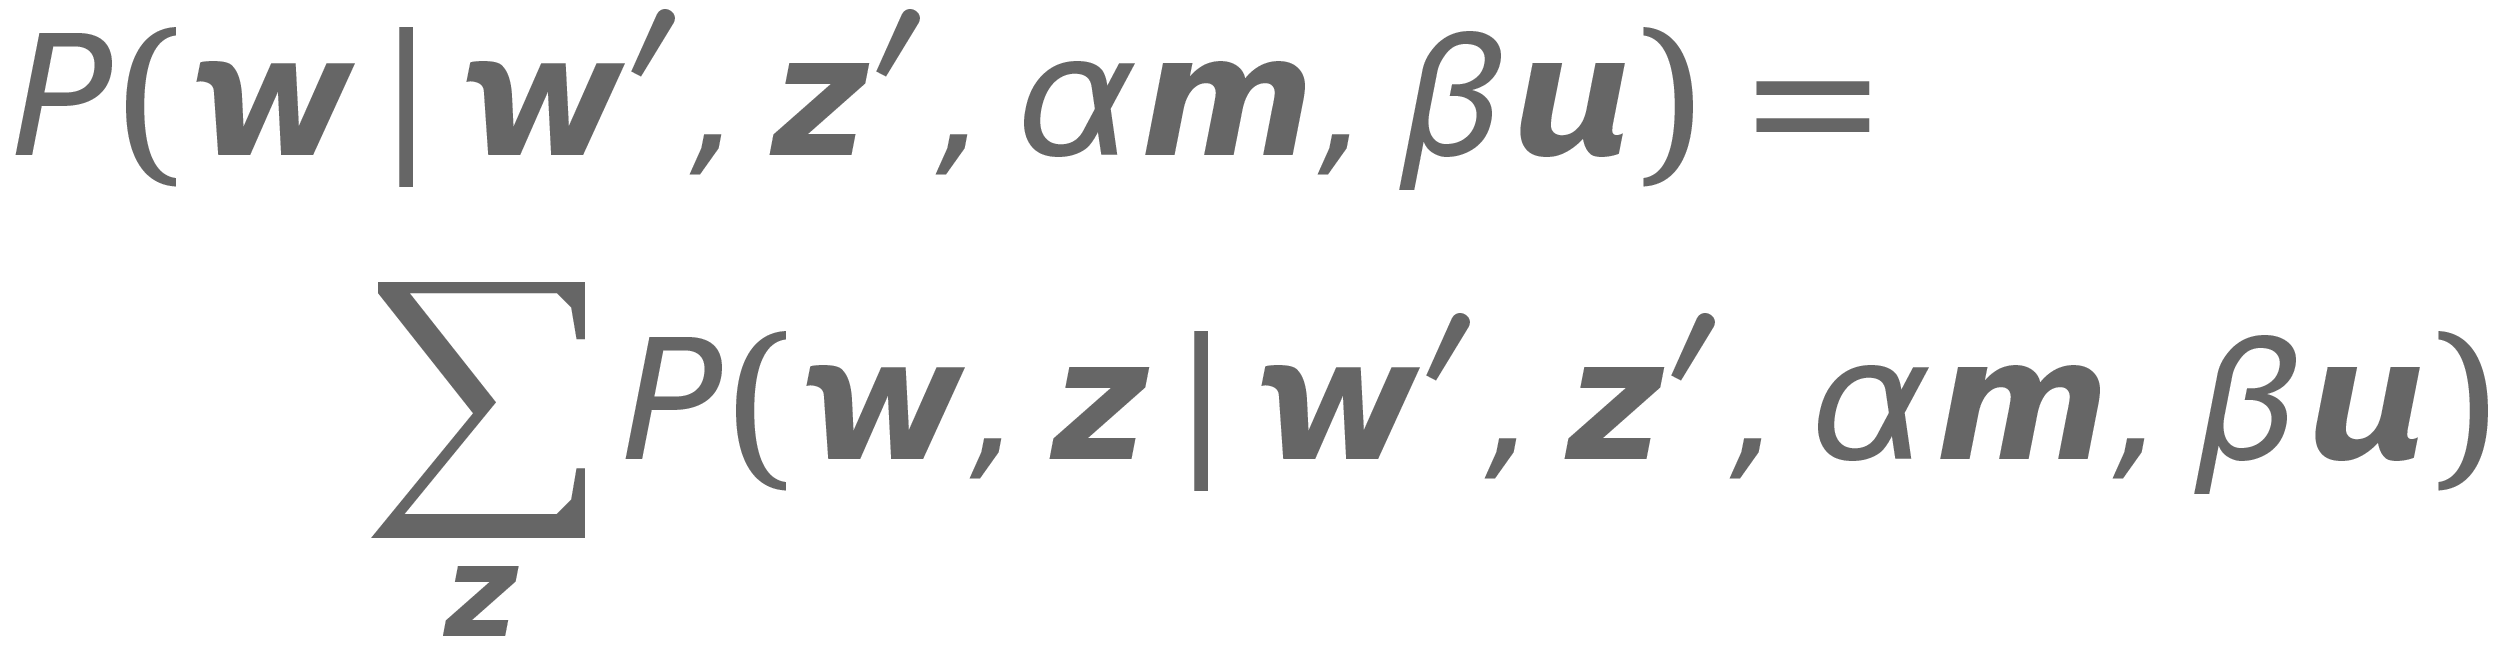
\includegraphics[width=0.5\linewidth]{topic_models/equations/evaluation} \\
How you compute it is important too~\cite{wallach-09b}
\end{center}

}

\frame{
  \frametitle{Word Intrusion}

  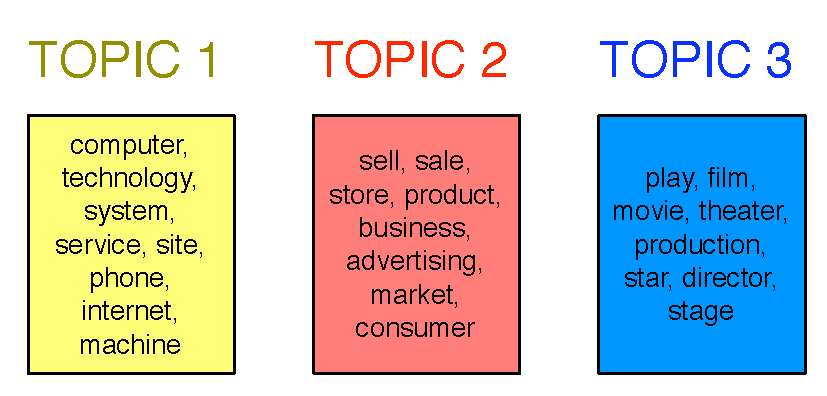
\includegraphics[width=\linewidth]{reading_tea_leaves/figures/nyt_topics_wide}
}


\frame{
  \frametitle{Word Intrusion}

  \begin{enumerate}
    \item Take the highest probability words from a topic

      \begin{block}{Original Topic}
        dog, cat, horse, pig, cow
      \end{block}
\pause
    \item Take a high-probability word from another topic and add it
      \begin{block}{Topic with Intruder}
        dog, cat, \alert<2->{apple}, horse, pig, cow
      \end{block}
\pause
     \item We ask users to find the word that doesn't belong
  \end{enumerate}
\begin{block}{Hypothesis}
If the topics are interpretable, users will consistently choose true intruder
\end{block}
}

\frame{
\frametitle{Word Intrusion}
\begin{center}
\only<1>{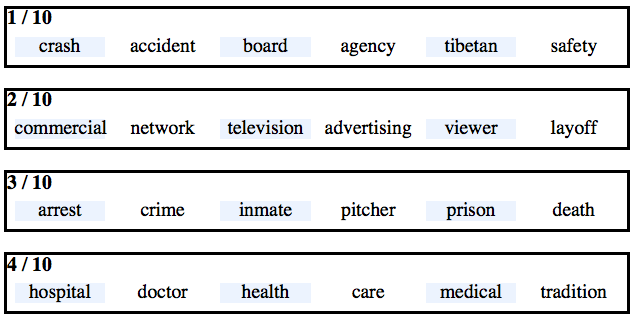
\includegraphics[width=\linewidth]{reading_tea_leaves/tasks/word1}  }
\only<2>{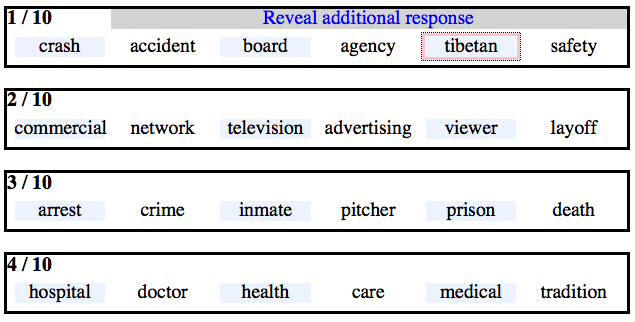
\includegraphics[width=\linewidth]{reading_tea_leaves/tasks/word2}  }
\pause
  \begin{itemize}
    \item Order of words was shuffled
    \item Which intruder was selected varied
    \item Model precision: percentage of users who clicked on intruder
  \end{itemize}

\end{center}
}

\frame{
\frametitle{Word Intrusion: Which Topics are Interpretable?}
  \begin{block}{New York Times, 50 LDA Topics}
    \begin{center}
      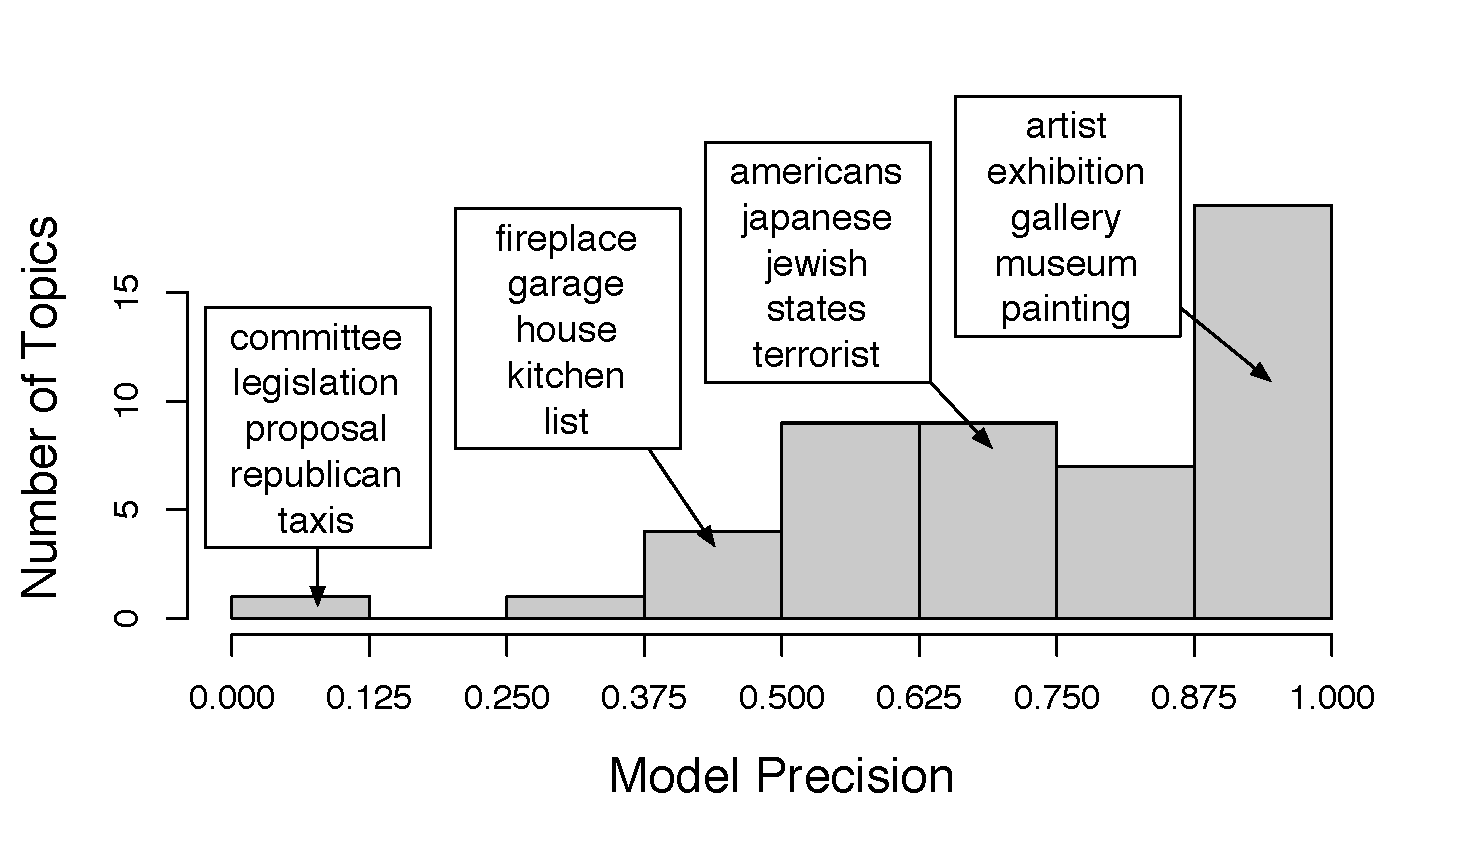
\includegraphics[width=0.8\linewidth]{reading_tea_leaves/figures/topic_precision}
    \end{center}
  \end{block}
  \begin{center}
    Model Precision: percentage of correct intruders found
  \end{center}
}



\frame{

\frametitle{Interpretability and Likelihood}
\begin{center}
\only<1>{Model Precision on New York Times}
\only<2>{Topic Log Odds on Wikipedia}
\end{center}

\begin{columns}
\column{.85\linewidth}
\begin{flushright}
  \only<1>{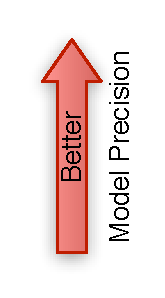
\includegraphics[scale=\graphscale]{reading_tea_leaves/tasks/mp}}
  \only<2>{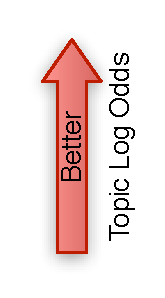
\includegraphics[scale=\graphscale]{reading_tea_leaves/tasks/tlo}}
  \only<1>{
\includegraphics[scale=\graphscale]{reading_tea_leaves/tasks/mp_y}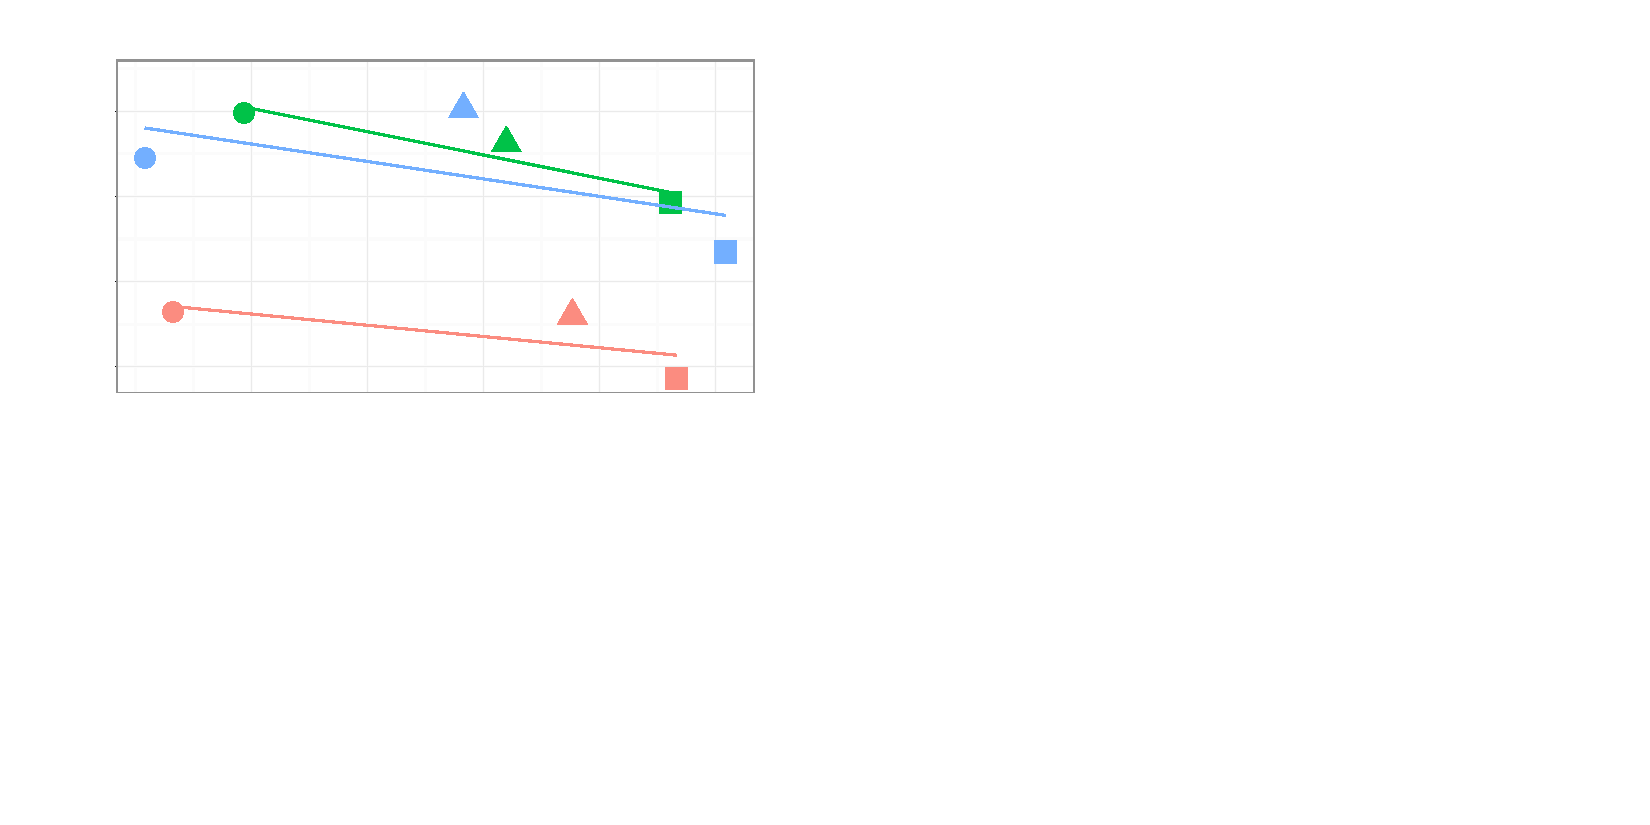
\includegraphics[scale=\graphscale]{reading_tea_leaves/tasks/nyt_mp}}
  \only<2>{
\includegraphics[scale=\graphscale]{reading_tea_leaves/tasks/tlo_y}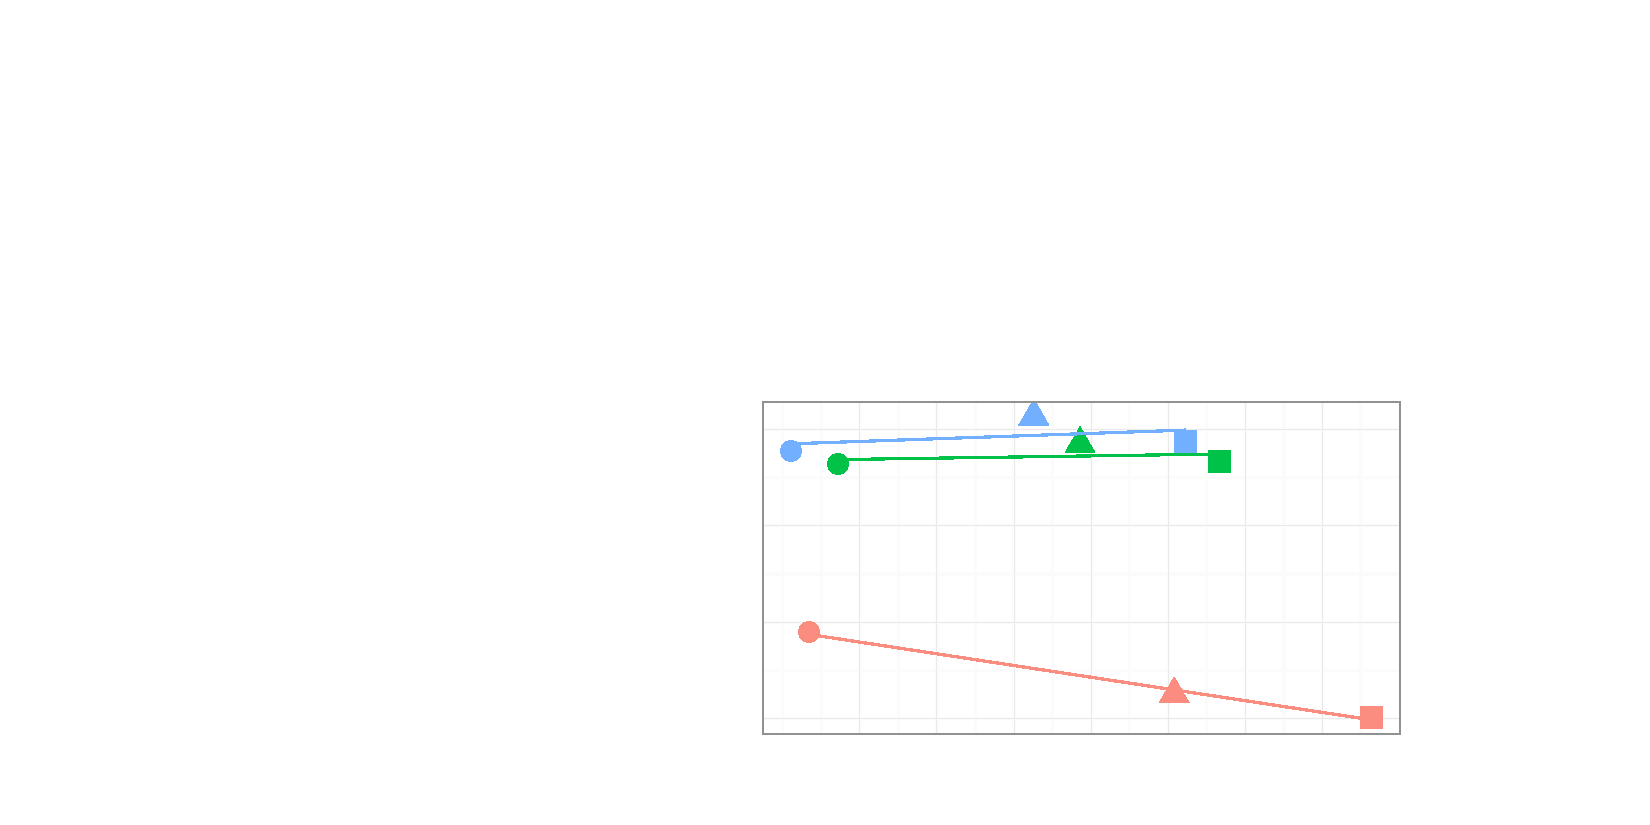
\includegraphics[scale=\graphscale]{reading_tea_leaves/tasks/wiki_tlo}} \\
  \only<1>{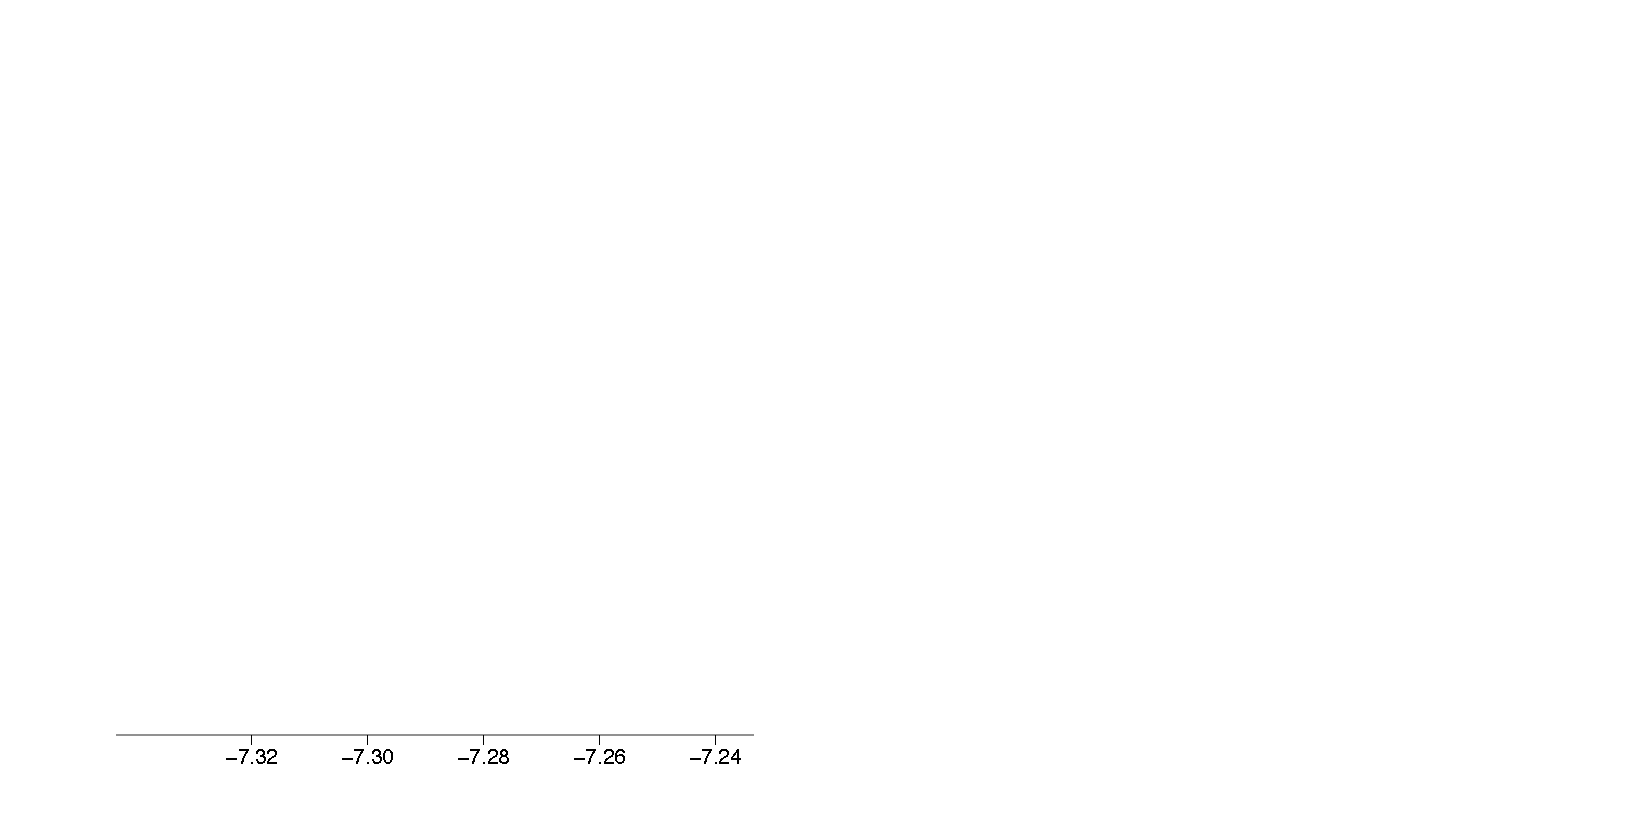
\includegraphics[scale=\graphscale]{reading_tea_leaves/tasks/nyt_x}}
  \only<2>{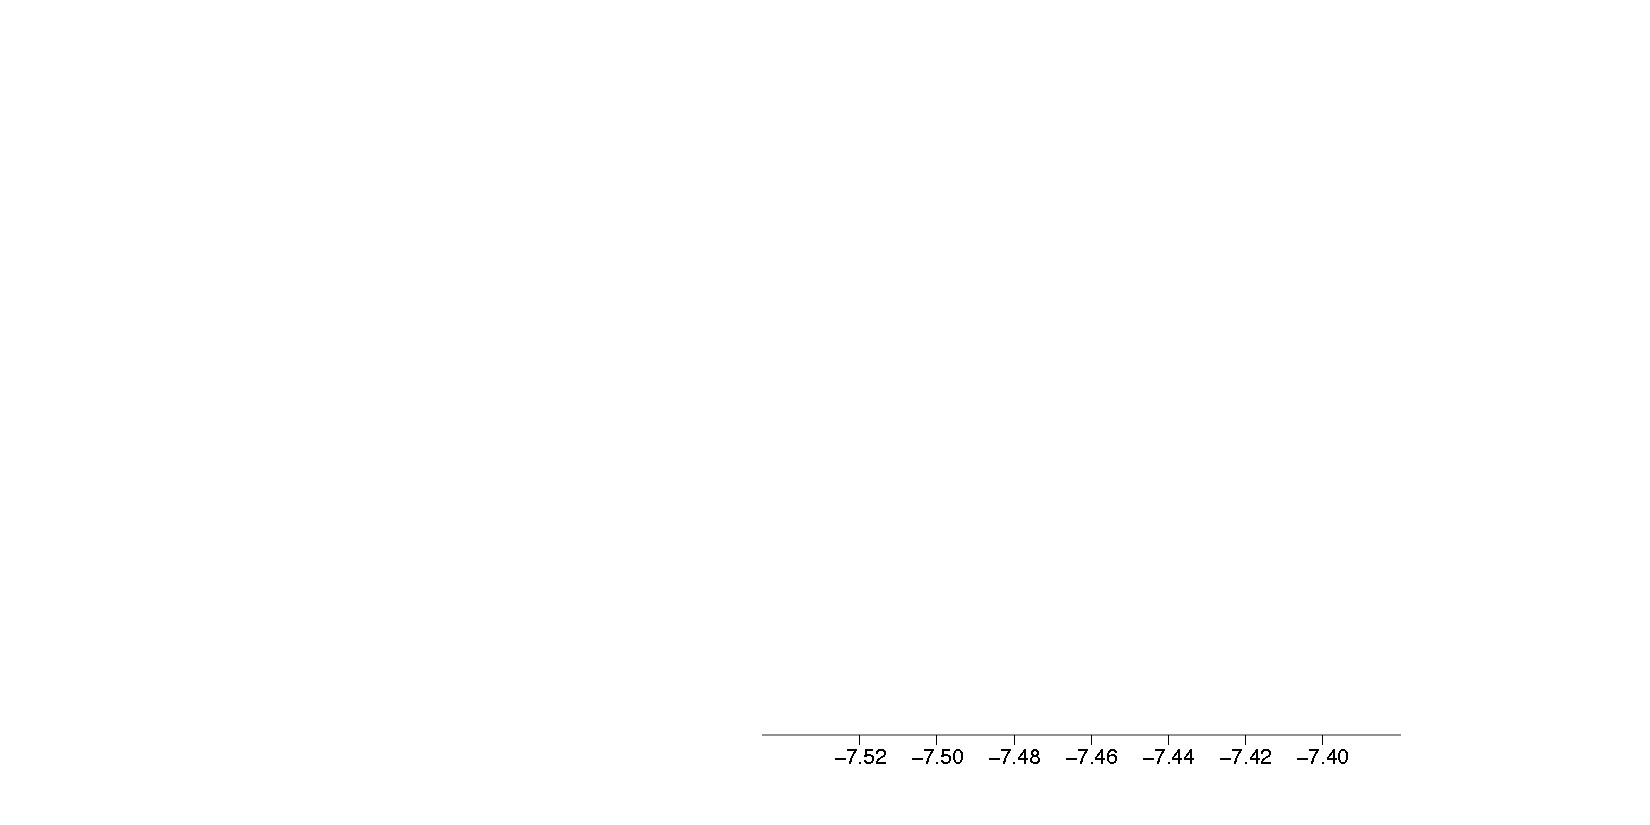
\includegraphics[scale=\graphscale]{reading_tea_leaves/tasks/wiki_x}}
\end{flushright}
\column{.15\linewidth}
  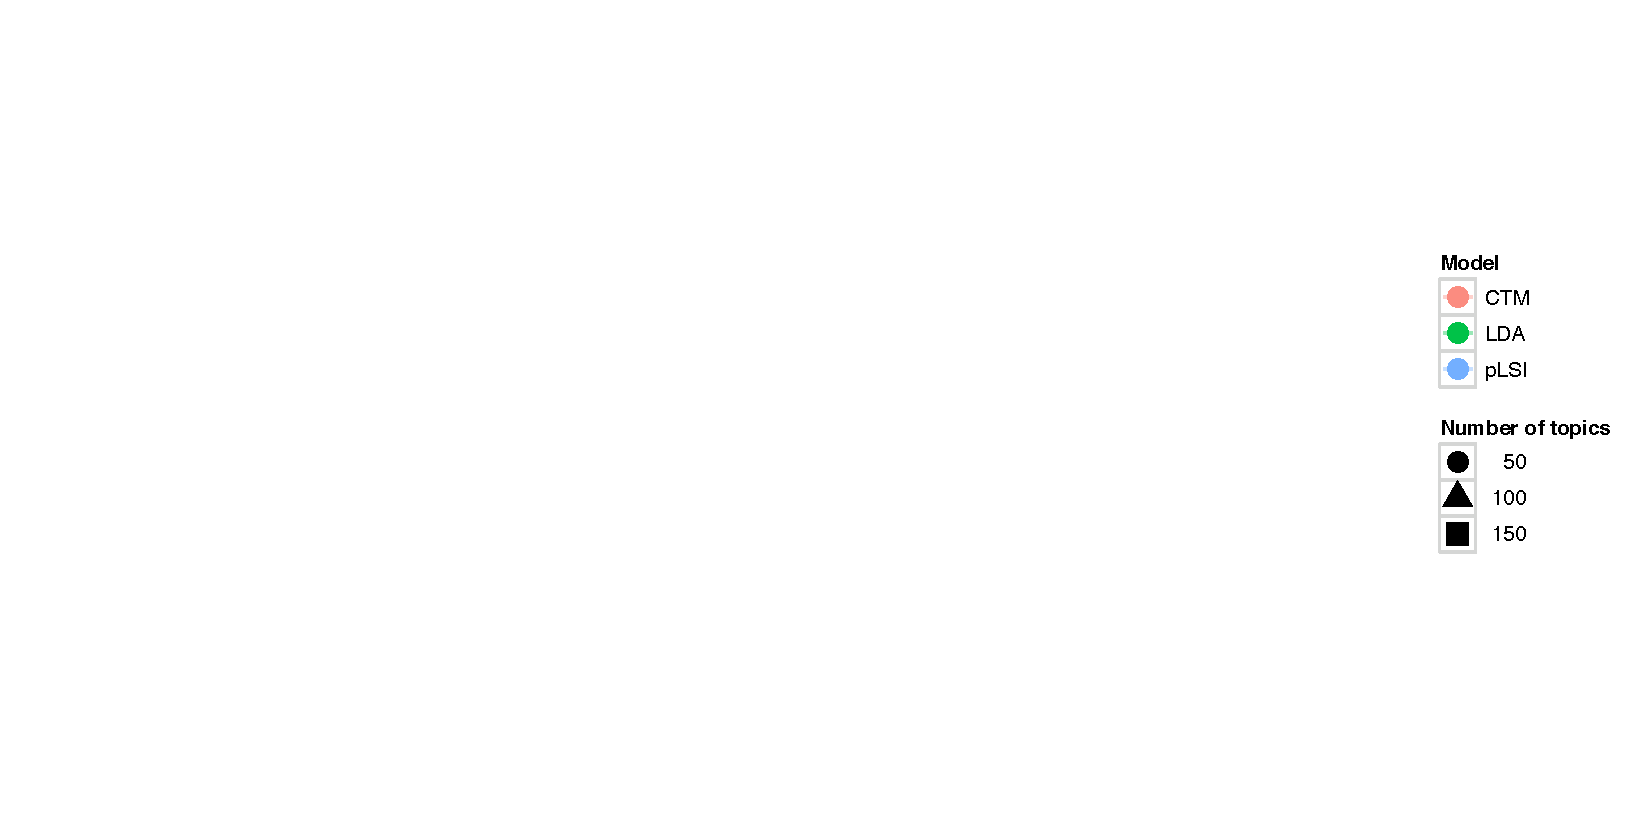
\includegraphics[scale=\graphscale]{reading_tea_leaves/tasks/legend}
\end{columns}
\vspace{-0.75cm}
\begin{center}
  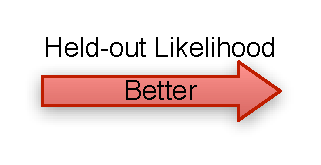
\includegraphics[scale=\graphscale]{reading_tea_leaves/tasks/held-out} \\
\only<1> {within a model, higher likelihood $\not =$ higher interpretability}
\only<2> {across models, higher likelihood $\not =$ higher interpretability}
\end{center}
}


\begin{frame}
  \frametitle{Evaluation Takeaway}

  \begin{itemize}
    \item Measure what you care about~\cite{chang-09c}
      \item If you care about prediction, likelihood is good
\item If you care about a particular task, measure that
    \end{itemize}

\end{frame}

\fi


\frame{
	\frametitle{Why topic models?}
	
	\begin{columns}
	
	\column{.5\linewidth}
	
	\begin{itemize}
		\item Facilitating distant reading: Matt Jockers (English literature), Robert Nelson (civil war journalism), David Mimno (classics journals)
		\item Applications beyond text~\cite{feifei-05,airoldi-08,hu-09}
	\end{itemize}
	
		\begin{flushright}
      			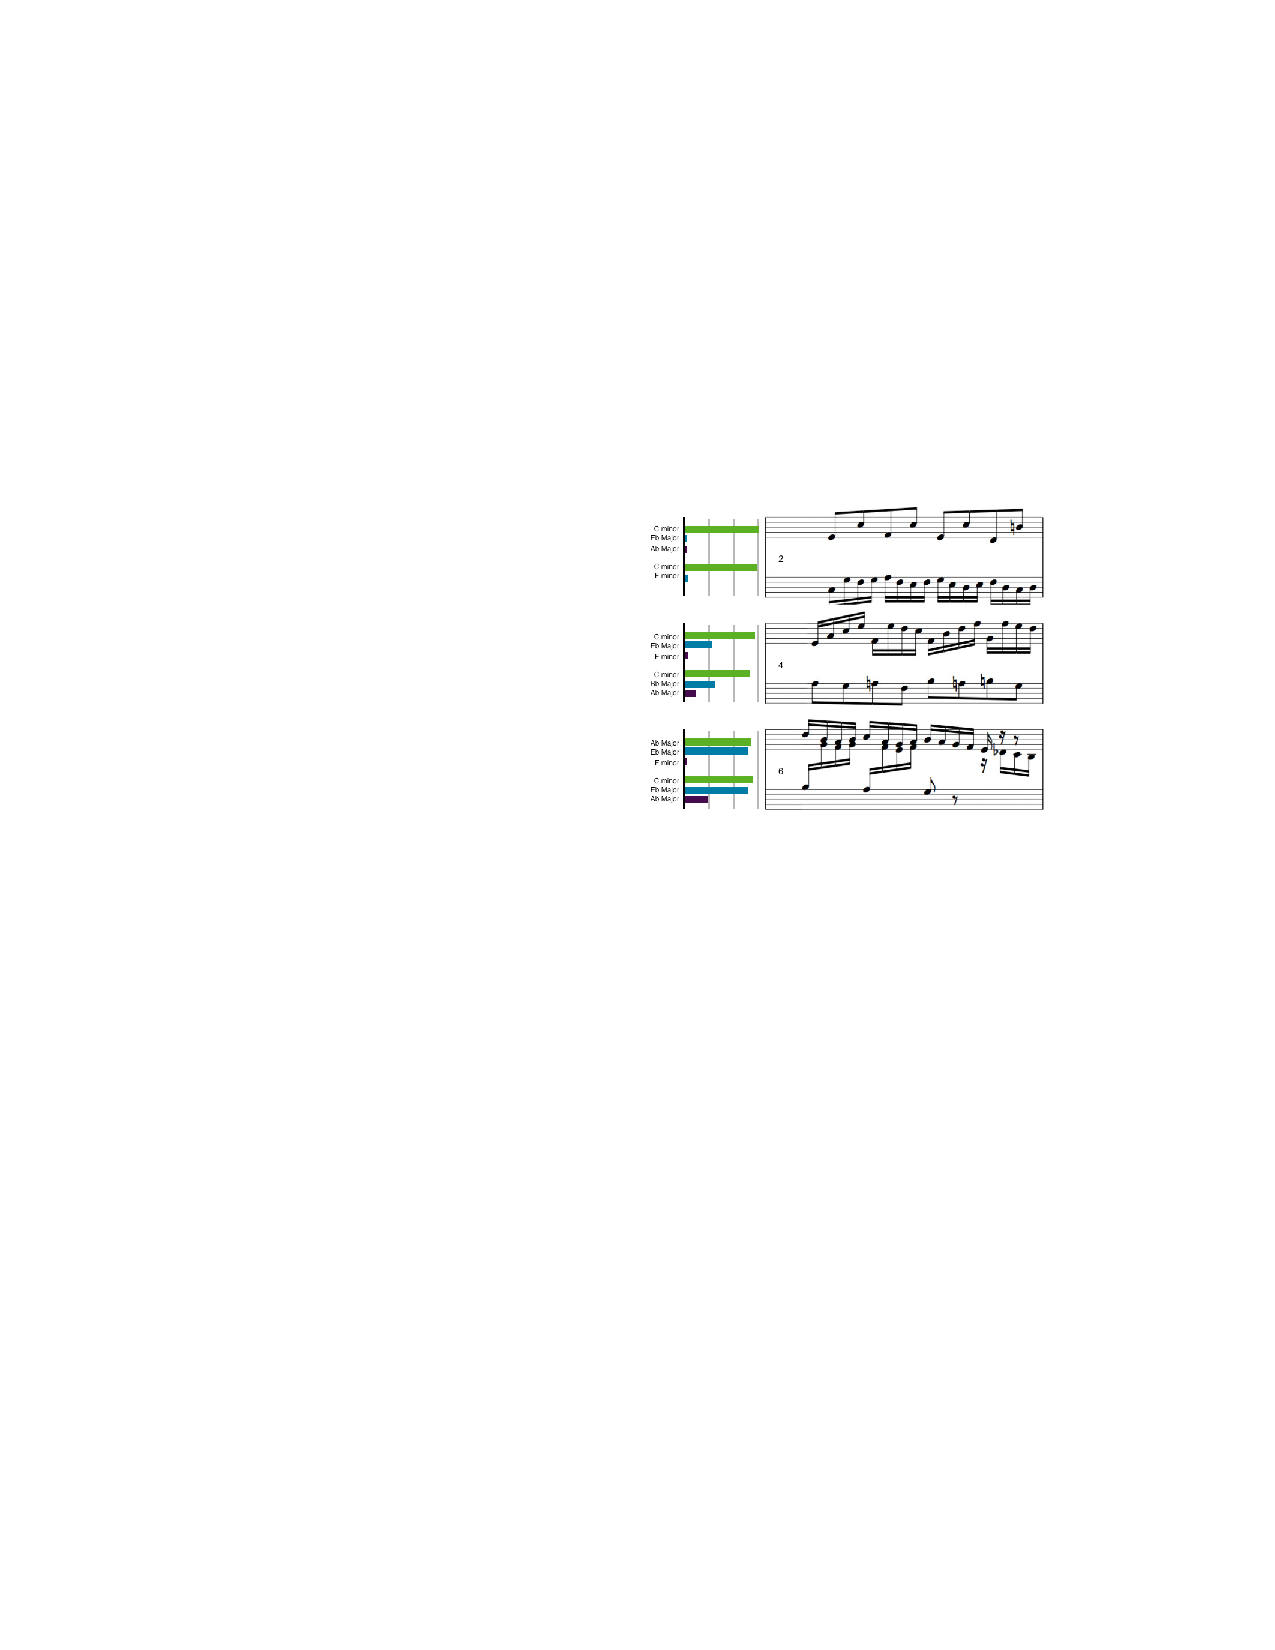
\includegraphics[width=3cm]{topic_models/hu} 
		\end{flushright}
	
	\column{.4\linewidth}

		\begin{center}
			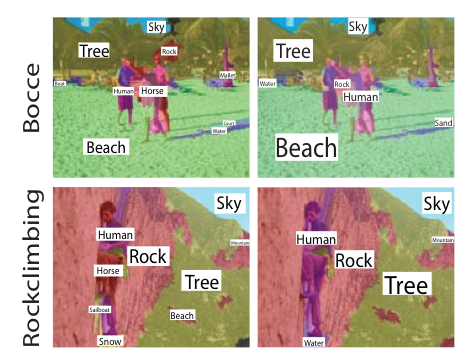
\includegraphics[width=4cm]{topic_models/feifei} 
			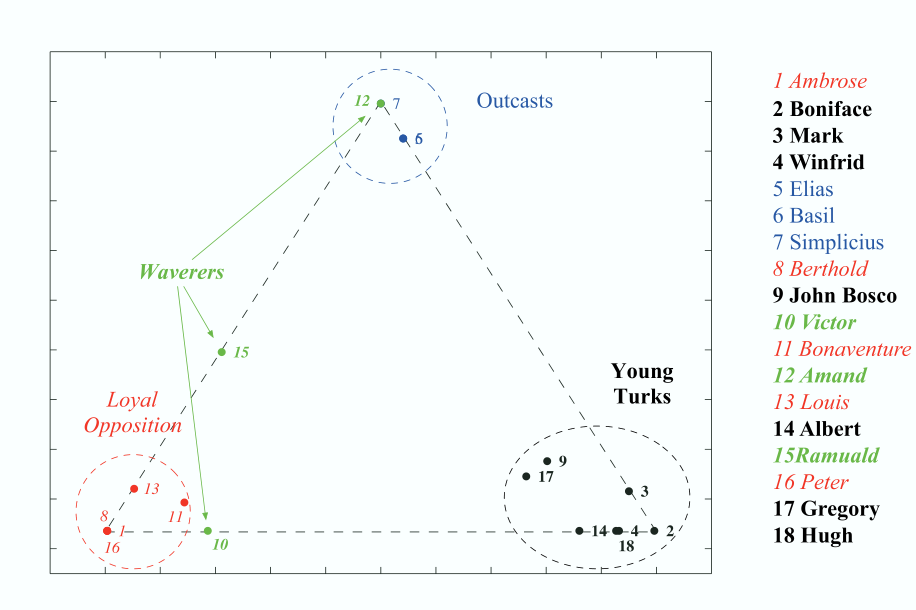
\includegraphics[width=4cm]{topic_models/socialnetworks} 
		\end{center}	
	
	\end{columns}
}

\frame{

\begin{columns}

\column{.5\linewidth}

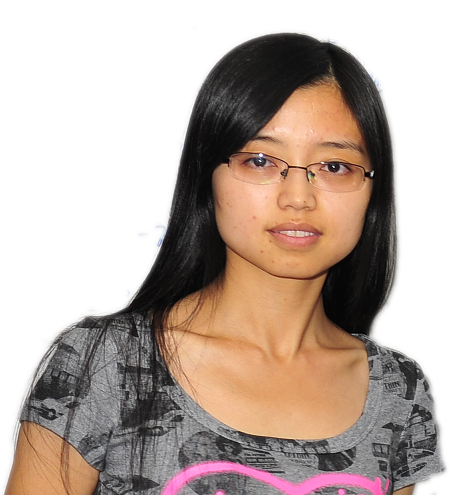
\includegraphics[width=.8\linewidth]{general_figures/yuening}

\column{.5\linewidth}

\begin{block}{Interactive Topic Modeling}
Yuening Hu, Jordan Boyd-Graber, and Brianna Satinoff.  Association for Computational Linguistics, 2011.
\end{block}

\end{columns}

}

\section{Interactive Topic Models}

\frame{

	\frametitle{Why interactive?}
	
	\begin{itemize}
		\item Correct obvious errors easily
		\item Builds better intuitions
		\item ``Buy in'' 		
		\item Better downstream models
	\end{itemize}

}



\newcommand{\itmspace}[0]{\hspace{2cm}}

\frame{

	\frametitle{What's the Problem?}

\begin{columns}
	\column{.4\linewidth}

	\begin{center}
	\begin{tabular}{cc}
		\alert<2>{shuttle} & \alert<2>{NASA} \\
		\alert<2>{launch} & telescope \\
		racket & quasar \\
		battledor & saturn \\
		backhand & space \\
		astronaut & moon \\
	\end{tabular}
	\end{center}

\column{.6\linewidth}

\only<2->{\danquote{Shuttle, launch, and NASA should be together!}}

\end{columns}

}

\frame{

\frametitle{What's the problem?}

\begin{columns}

\column{.4\linewidth}
\begin{center}
\begin{tabular}{ccc}
& \only<2->{\itmspace}\color<2->{red}{bladder} & \\
& \only<3->{\hspace{-2cm}} \color<3->{blue}{spinal\_cord}  & \\
& \only<3->{\hspace{-2cm}} \color<3->{blue}{sci} & \\
& \only<3->{\hspace{-2cm}}\color<3->{blue}{spinal\_cord\_injury} & \\
& \only<3->{\hspace{-2cm}}\color<3->{blue}{spinal} & \\
& \only<2->{\itmspace}\color<2->{red}{urinary} & \\
& \only<2->{\itmspace}\color<2->{red}{urothelial} & \\
& \only<3->{\hspace{-2cm}}\color<3->{blue}{cervical} & \\
& injury & \\
& recovery & \\
& \only<2->{\itmspace}\color<2->{red}{urinary\_tract} & \\
& locomotor & \\
& \only<3->{\hspace{-2cm}}\color<3->{blue}{lumbar} & \\
\end{tabular}
\end{center}

\column{.6\linewidth}

\danquote{These words don't belong together!}

\end{columns}

}


\frame{
	\frametitle{How to fix it?}

\begin{columns}

\column{.4\linewidth}

\begin{itemize}
	\item The topics in a topic model are \only<2->{\alert<2>{uncorrelated}} distributions over words
	\only<3->{
	\item The advice you get can be encoded as correlations
		\begin{itemize}
			\alert<4>{\item Positive correlations}
			\alert<5>{\item Negative correlations}
		\end{itemize}
	}
	\only<6->{
	\item Technical details: Dirichlet Forest~\cite{boyd-graber-07,andrzejewski-09}
	}
\end{itemize}

\column{.6\linewidth}

	\only<1-2>{	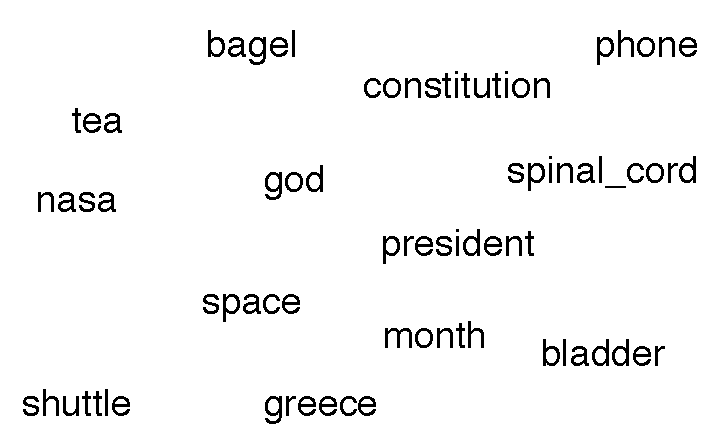
\includegraphics[width=\linewidth]{interactive_topic_models/constraints_1}     }
	\only<3-4>{	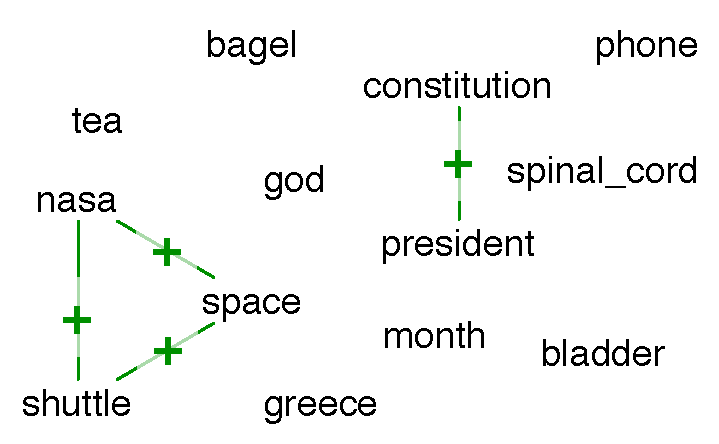
\includegraphics[width=\linewidth]{interactive_topic_models/constraints_2}     }
	\only<5->{	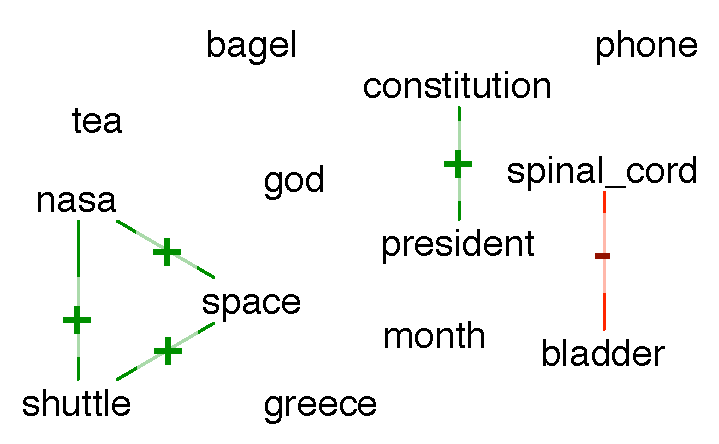
\includegraphics[width=\linewidth]{interactive_topic_models/constraints_3}     }
\end{columns}

}

\ifitmtree

\frame{

	\frametitle{Tree-based Generative Process}

	\begin{itemize}
		\item In LDA, a topic is a multinomial distribution over words
		\item Here, \emph{each topic} is a tree
		\begin{itemize}
			\item Each word is a leaf
			\item Start at root node
			\item Proceed down tree node by node until you reach a leaf
		\end{itemize}
	\end{itemize}
}


\frame{

	\frametitle{Example of Priors}

	\begin{center}
		\only<1>{ 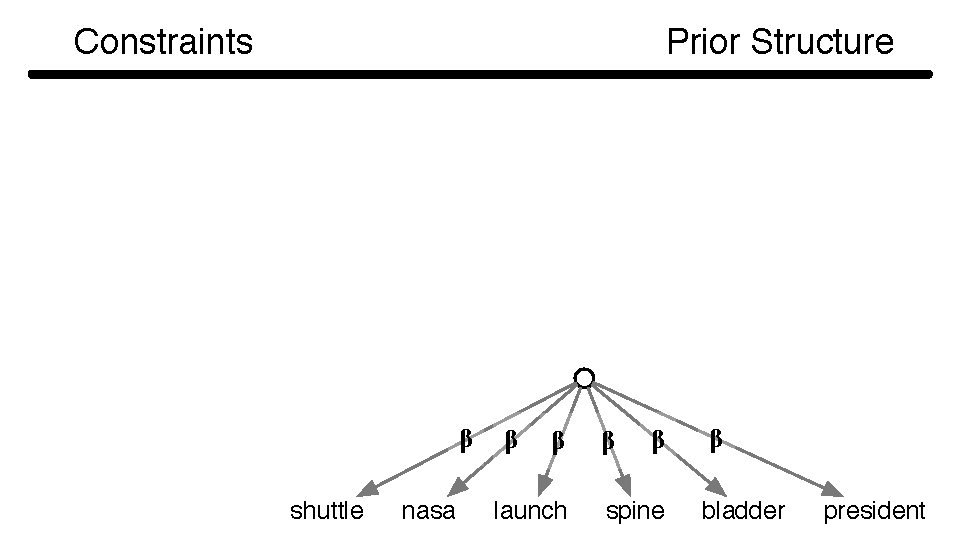
\includegraphics[width=.8\linewidth]{interactive_topic_models/tree_constraints_0} }
		\only<2>{ \includegraphics[width=.8\linewidth]{interactive_topic_models/tree_constraints_1} }
		\only<3>{ \includegraphics[width=.8\linewidth]{interactive_topic_models/tree_constraints_2} }
	\end{center}

	\begin{columns}

		\column{.5\linewidth}

			\only<2>{

			\begin{itemize}
				\item For negative correlations $\tau << \beta$
				\item Encourages very, very sparse distributions
			\end{itemize}
				\includegraphics[width=.7\linewidth]{interactive_topic_models/uniform_dirichlet}


			}


			\only<3>{

			\begin{itemize}
				\item For positive correlations $\eta >> \beta$
				\item Encourages uniform distributions
			\end{itemize}
				\includegraphics[width=.7\linewidth]{interactive_topic_models/sparse_dirichlet}


			}

		\column{.5\linewidth}

	\end{columns}

}

\fi

\frame{
	\frametitle{How to incorporate feedback?}

	\begin{columns}

	\column{.5\linewidth}

		\begin{columns}

			\column{.6\linewidth}

			\includegraphics[width=\linewidth]{topic_models/nyt_topics}


			\column{.4\linewidth}
			\begin{center}
				\only<2->{\includegraphics[width=.6\linewidth]{general_figures/arrow_right_down} \\}
				\only<2->{\includegraphics[width=.6\linewidth]{general_figures/milkman_dan} \\}
				\invisible<-2>{\includegraphics[width=.6\linewidth,angle=270]{general_figures/arrow_right_down}}
			\end{center}

		\end{columns}

	\column{.5\linewidth}

	\begin{enumerate}
		\item Fit initial topic modeling
			\pause
		\item Get feedback from user
			\pause
		\item Incrementally relearn model
			\begin{itemize}
				\item Replace the model with a correlated one
				\item Keep computation \alert<4>{fast and consistent}
			\end{itemize}
	\end{enumerate}

	\end{columns}

}



\ifhighlevel

\else

\frame{
	\frametitle{Forgetting is everything}

	\begin{itemize}
		\item Just start over?
			\begin{itemize}
				\item More expensive computation
				\item Might create more problems
				\item Bad user experience
			\end{itemize}
		\item View problem as online inference~\cite{yao-09}
		\item Suggestions reflect errors
		\item ``Forget'' problems
		\item Pretend you're seeing it for the first time
	\end{itemize}
}


\frame{
	\frametitle{Inference}


	\begin{center}

	\only<1> {   \includegraphics[width=.8\linewidth]{topic_models/inference_0}  }
	\only<2> {   \includegraphics[width=.8\linewidth]{topic_models/inference_1}  }
	\only<3> {   \includegraphics[width=.8\linewidth]{topic_models/inference_2}  }
	\only<4> {   \includegraphics[width=.8\linewidth]{topic_models/inference_3}  }
	\end{center}

}

\frame{
	\frametitle{Inference}

	\begin{columns}

		\column{.5\linewidth}
		\begin{flushright}
			\only<1>{    \includegraphics[height=7cm]{interactive_topic_models/mcmc_state_0}    }
			\only<2>{    \includegraphics[height=7cm]{interactive_topic_models/mcmc_state_1}    }
			\only<3>{    \includegraphics[height=7cm]{interactive_topic_models/mcmc_state_2}    }
			\only<4>{    \includegraphics[height=7cm]{interactive_topic_models/mcmc_state_3}    }							\only<5>{    \includegraphics[height=7cm]{interactive_topic_models/mcmc_state_4}    }
			\only<6>{    \includegraphics[height=7cm]{interactive_topic_models/mcmc_state_5}    }
			\only<7>{    \includegraphics[height=7cm]{interactive_topic_models/mcmc_state_6}    }
			\only<8>{    \includegraphics[height=7cm]{interactive_topic_models/mcmc_state_7}    }
			\only<9>{    \includegraphics[height=7cm]{interactive_topic_models/mcmc_state_8}    }
			\only<10>{    \includegraphics[height=7cm]{interactive_topic_models/mcmc_state_9}    }							\only<11->{    \includegraphics[height=7cm]{interactive_topic_models/mcmc_state_a}    }
		\end{flushright}
		\column{.5\linewidth}

		\only<1> {  This toy example has all the problems from before!  }
		\only<2-6> {

		\includegraphics[width=\linewidth]{interactive_topic_models/constraints_4}

		\begin{block}{Negative Correlation}

		\begin{itemize}
			\item \emph{bladder} and \emph{spine} can't be together
			\item Idea 1: Forget {\bf terms}
		\end{itemize}


		\end{block}

		}

		\only<7-11> {

		\includegraphics[width=\linewidth]{interactive_topic_models/constraints_5}

		\begin{block}{Positive Correlation}
		\begin{itemize}
			\item \emph{shuttle} and \emph{nasa} should be together
			\item Idea 2: Forget {\bf documents} with terms
		\end{itemize}
		\end{block}

		}

	\end{columns}

}


\frame{
	\frametitle{Tricky details}

	\begin{itemize}
		\item Overlapping correlations
		\begin{itemize}
			\item Are positive correlations transitive (polysemy)
			\item Overlapping negative correlations require computing maximal cliques in complement graph
		\end{itemize}
		\item How do you do hyperparameter optimization?
		\pause
		\item For the rest of this talk, only {\bf positive} correlations and preset hyper parameters
	\end{itemize}
}

\fi

\renewcommand{\tb}[1]{\parbox{0.8\linewidth}{ \tiny{ #1 }} \vspace{.2cm} }

\frame{

\vspace{-1cm}

\begin{columns}

\column{.5\linewidth}

\begin{tabular}{l*{2}{c}r}
	Topic & Before \\
\hline

\alert<2>{{\bf 1}} & \tb{ \alert<2>{election, yeltsin, russian, political, party, democratic, russia,
  president, democracy, boris, country, south, years, month, government, vote,
  since, leader, presidential, military} } \\

2 & \tb{new, york, city, state, mayor, budget, giuliani, council, cuomo, gov,
  plan, year, rudolph, dinkins, lead, need, governor, legislature, pataki,
  david} \\

3 & \tb{nuclear, arms, weapon, defense, treaty, missile, world, unite, yet,
  soviet, lead, secretary, would, control, korea, intelligence, test, nation,
  country, testing} \\

4 & \tb{president, bush, administration, clinton, american, force, reagan, war,
  unite, lead, economic, iraq, congress, america, iraqi, policy, aid,
  international, military, see} \\

& \vdots \\

\alert<2>{{\bf 20}} & \tb{\alert<2>{soviet, lead, gorbachev, union, west, mikhail, reform, change, europe,
  leaders, poland, communist, know, old, right, human, washington, western,
  bring, party} }\\

\end{tabular}

\column{.5\linewidth}

\only<3> {

	\begin{block}{Suggestion}
	\emph{boris, communist, gorbachev, mikhail, russia,
  russian, soviet, union, yeltsin }
	\end{block}

}

\only<4-> {

\begin{tabular}{l*{2}{c}r}
	Topic & After \\
\hline

\alert<5>{{\bf 1}} & \alert<5>{\tb{election, democratic, south, country, president, party, africa, lead,
  even, democracy, leader, presidential, week, politics, minister, percent,
  voter, last, month, years} } \\

\alert<6>{2} & \tb{new, york, city, state, mayor, budget, council, giuliani, gov, cuomo,
  year, rudolph, dinkins, legislature, plan, david, governor, pataki, need, cut}
\\

\alert<6>{3} & \tb{nuclear, arms, weapon, treaty, defense, war, missile, may, come, test,
  american, world, would, need, lead, get, join, yet, clinton, nation} \\

\alert<6>{4} & \tb{president, administration, bush, clinton, war, unite, force, reagan,
  american, america, make, nation, military, iraq, iraqi, troops, international,
  country, yesterday, plan} \\

   & \vdots \\

\alert<4>{ {\bf 20} } & \alert<4> {\tb{soviet, union, economic, reform, yeltsin, russian, lead, russia,
  gorbachev, leaders, west, president, boris, moscow, europe, poland, mikhail,
  communist, power, relations} } \\

\end{tabular}

}

\end{columns}

}

\providecommand{\blue}[1]{{\color{blue}{#1}}}
\providecommand{\red}[1]{{\color{red}{#1}}}
\providecommand{\green}[1]{{\color{green}{#1}}}

\begin{frame}

\frametitle{Example: Negative Constraint}

\begin{columns}

\column{.4\linewidth}

\begin{tabular}{l*{2}{c}r}
	Topic & Words \\
\hline

{\bf 318} & \tb{\red{bladder}, sci, \blue{spinal\_cord}, \blue{spinal\_cord\_injury}, \blue{spinal}, \red{urinary}, \red{urinary\_tract}, \red{urothelial},\blue{injury}, \blue{motor}, \blue{recovery}, \blue{reflex}, \blue{cervical}, \red{urothelium}, \blue{functional\_recovery}} \\

\end{tabular}

\column{.1\linewidth}

\column{.4\linewidth}

\only<3->{
\begin{tabular}{l*{2}{c}r}
	Topic & Words \\
\hline

{\bf 318} & \tb{sci, \blue{spinal\_cord}, \blue{spinal\_cord\_injury}, \blue{spinal}, \blue{injury}, \blue{recovery}, \blue{motor}, \blue{reflex}, \red{urothelial}, \green{injured}, \blue{functional\_recovery}, \green{plasticity}, \green{locomotor}, \blue{cervical}, \green{locomotion}}\\

\end{tabular}
}

\end{columns}

\only<2->{
\begin{block}{Negative Constraint}
  spinal\_cord, bladder
\end{block}

}

\end{frame}




\begin{frame}

        \frametitle{Experiments}

\begin{columns}

\column{.5\linewidth}

  \begin{itemize}
   \item Simulating users through classifying social media
     \begin{itemize}
       \item Investigating different learning strategies
       \item How much to forget
     \end{itemize}
   \end{itemize}

\column{.5\linewidth}

\begin{center}
\includegraphics[width=\linewidth]{interactive_topic_models/ablation_30_topics}
\end{center}

\end{columns}

\begin{itemize}
    \item User study: mechanical Turk
      \begin{itemize}
        \item We can't do everything users want: proper names, mac vs. pc
        \item Users are senstive to polysemy (``msg'': food or e-mail)
      \end{itemize}
    \item User study: exploring congressional debates
      \begin{itemize}
        \item Collaboration with social scientists
        \item Interactivity makes people use topic models more
       \end{itemize}
  \end{itemize}


\end{frame}

% -------------------------
% Old version

% \frame{
% 	\frametitle{Interactive Topic Models in the Wild \dots}
% \begin{center}
% 	\only<1>{    \includegraphics[width=\linewidth]{interactive_topic_models/turk_topic}    }
% 	\only<2>{    \includegraphics[width=\linewidth]{interactive_topic_models/turk_sel_constraint}    }
% 	\only<3>{    \includegraphics[width=\linewidth]{interactive_topic_models/turk_add_link}    }
% 	\only<4>{    \includegraphics[width=\linewidth]{interactive_topic_models/best_mturk_rel_error}    }

% 	\begin{block}{}
% 		Documents were 20 Newsgroups
% 	\end{block}
% \end{center}
% }



\iflong

\frame{
	\frametitle{What people did \dots}


	\begin{itemize}
		\item Inscrutable
			\begin{itemize}
				\item better, people, right, take, things
				\item fbi, let, says
			\end{itemize}
		\item Collocations
			\begin{itemize}
				\item jesus, christ
				\item solar, sun
				\item even, number
				\item book, list
			\end{itemize}
		\item Common instances (e.g. first names)
		\item Not all were successful: mac, windows

	\end{itemize}

}


\frame{

	\frametitle{Future steps}

	\begin{itemize}
		\item Speeding up
		\item Suggesting correlations
		\item Incorporating other domain knowledge
		\item Interactive vocabulary
		\item Other domains
		\item Incorporating this analysis in other models
	\end{itemize}

}

\fi





\begin{frame}{}

  \begin{columns}
    \column{.5\linewidth}
      \includegraphics[width=.9\linewidth]{general_figures/an}
    \column{.5\linewidth}
    \begin{block}{Tea Party in the House: A Hierarchical Ideal Point Topic Model
  and Its Application to Republican Legislators in the 112\textsuperscript{th} Congress}
  
  Viet-An Nguyen (UMD), Kristina Miler (UMD), Jordan Boyd-Graber (UCB), and Philip Resnik (UMD)
  
    \end{block}
      \begin{itemize}
        \item Former PhD student at Maryland
        \item Now at Facebook
        \item Application of ITM
      \end{itemize}
  \end{columns}

\end{frame}

\section[Multi-dimensional Ideal Points from Roll-call Votes and Text]{Multi-dimensional Ideal Points from Roll-call Votes and Text}%


\section{Motivation}

\begin{frame}{Representing Elected Officials: Ideal Points}
  \gfx{dw_nominate}{.7}
  \pause
  An essential tool in political science: distinguish trends and characterize subgroups
\end{frame}


\frame{
\frametitle{Evaluation: Tea Party in the House}
    \begin{block}{The Tea Party}
    \small
    \begin{itemize*}
      \item Recent American political movement supporting more freedom, smaller government, lower tax
      \item Played an important role in recent electoral politics, especially within the Republican
      Party
      \item Organizations:
      \begin{itemize}
        \item Institutional: Tea Party Caucus
        \item Other: Tea Party Express, Tea Party Patriots, Freedom Works
      \end{itemize}
      \item ``\textbf{Conventional views of ideology as a single--dimensional, left�-right
          spectrum experience great difficulty in understanding or explaining the Tea Party.}''

        \hfill \cite[ARPS]{CarminesARPS15}
    \end{itemize*}
    \end{block}

    \pause
    \vspace{-.2cm}
    \begin{block}{Goal}
    \small
    \begin{itemize*}
      \item Explain Tea Partiers in terms of issues and votes
      \item Identify Tea Partiers from their rhetoric
    \end{itemize*}
    \end{block}
}


\begin{frame}{Not everyone has a voting record}

  \begin{columns}
    \column{.5\linewidth}
    \begin{itemize}
      \item Ideal points estimated based on voting record
      \item Not all candidates have a voting record
        \begin{itemize}
          \item Governors
          \item Entertainers
          \item CEOs
        \end{itemize}
        \pause
       \item But all politicians---by definition---talk
      \end{itemize}
      \column{.25\linewidth}
        \gfx{carson}{.75}
        \gfx{fiorina}{.75}
      \column{.25\linewidth}
        \gfx{walker}{.75}
        \gfx{schwarzenegger}{.75}
  \end{columns}

\end{frame}

\begin{frame}{Let's use whatever data we have}

\begin{columns}
  \column{.6\linewidth}
  \gfx{carson_twitter}{.95}
  \column{.4\linewidth}
  A single model that uses:
  \begin{itemize}
    \item Bill text
    \item Votes
    \item Commentary
  \end{itemize}
  to map political actors to the same continuous space.
\end{columns}
\end{frame}

\section{Ideal Point Review}

\frame{
    \frametitle{One-dimensional Ideal Point using Votes}
    \begin{figure}
      \centering
        \only<1>{\includegraphics[width=.9\textwidth]{teaparty/figures/s5/1_votes}}%
        \only<2>{\includegraphics[width=.9\textwidth]{teaparty/figures/s5/2_onedim_ip_eqn}}%
        \only<3>{\includegraphics[width=.9\textwidth]{teaparty/figures/s5/3_onedim_ip_eqn_explained}}%
        \only<4->{\includegraphics[width=.9\textwidth]{teaparty/figures/s5/3a_onedim_ip_eqn_highlighted}}%
    \end{figure}
    \vspace{-.3cm}
    \hfill \tiny{\cite{Poole:AJPS85}}

    \vspace{-0.5cm}

    \begin{columns}
      \column{\textwidth}
        \begin{center}
            \only<1-3>{\includegraphics[width=.8\textwidth]{teaparty/figures/s5/dimensions_0}}%
            \only<4>{\includegraphics[width=.8\textwidth]{teaparty/figures/s5/dimensions_1}}%
            \only<5>{\includegraphics[width=.8\textwidth]{teaparty/figures/s5/dimensions_2}}%
        \end{center}
    \end{columns}
}%

\frame{
    \frametitle{Multi-dimensional Ideal Point using Votes}
    \begin{figure}
      \centering
        \only<1>{\includegraphics[width=.8\textwidth]{teaparty/figures/s5/4_multdim_ip_eqn}}%
        \only<2>{\includegraphics[width=.8\textwidth]{teaparty/figures/s5/5_multdim_ip_eqn_explained}}%
        \only<3->{\includegraphics[width=.8\textwidth]{teaparty/figures/s5/5a_multdim_ip_eqn_highlighted}}%
    \end{figure}
    \vspace{-.2cm}    
    \hfill \tiny{\cite{Heckman:NBER96,Jackman:PA01,Clinton:APSR04}}    
    \vspace{-.3cm}
    \begin{figure}
        \only<1-2>{\includegraphics[width=.7\textwidth]{teaparty/figures/s5/dimensions_0}}%
        \only<3>{\includegraphics[width=.7\textwidth]{teaparty/figures/s5/dimensions_3}}%
        \only<4>{\includegraphics[width=.7\textwidth]{teaparty/figures/s5/dimensions_4}}%
    \end{figure}
}%

\frame{
    \frametitle{Multi-dimensional Ideal Point using Votes \& \textbf{Text}}
    \begin{figure}
      \centering
        \only<1>{\includegraphics[width=.8\textwidth]{teaparty/figures/s5/1a_votes_text}}%
        \only<2>{\includegraphics[width=.8\textwidth]{teaparty/figures/s5/6_multdim_ip_text_eqn}}%
        \only<3->{\includegraphics[width=.8\textwidth]{teaparty/figures/s5/7_multdim_ip_text_eqn_explained}}%
    \end{figure}
    \vspace{-.3cm}
    \hfill \tiny{} \cite{Gerrish:NIPS12,Bonica:AJPS13:ideology,Lauderdale:AJPS14,Sim:AAAI15:utility}
    \begin{figure}
        \only<1-3>{\includegraphics[width=.7\textwidth]{teaparty/figures/s5/dimensions_4}}%
        \only<4->{\includegraphics[width=.7\textwidth]{teaparty/figures/s5/dimensions_5}}%
    \end{figure}
}%

\begin{frame}{First-level topics from Political Scientists}

\begin{columns}
	\column{.5\linewidth}
		\begin{itemize}
			\item Government 
			\item Trade
			\item Defense
			\item Law and Crime 
			\item Transportation 		
			\item Parks and Lands 										
		\end{itemize}
	\column{.5\linewidth}
		\begin{itemize}
			\item Energy 
			\item Environment 
			\item Education 
			\item Labor Issues 
			\item Health 
			\item Rights and Liberties 												
		\end{itemize}
	
\end{columns}

\end{frame}

\section{Hierarchical Ideal Point Topic Model}

\frame{
    \frametitle{Our approach: Hierarchical Ideal Point Topic Model}
    \begin{figure}
    \centering
      \includegraphics[width=\textwidth]{teaparty/figures/s5/expected_output}
    \end{figure}
}

\frame{
    \frametitle{Hierarchical Ideal Point Topic Model: Overview}
    \only<1-5>{
    \begin{block}{Using both votes and text to learn}
        \begin{itemize}
          \item Two-level topic hierarchy:
            \only<2>{
            \begin{itemize} 
            \item \alert<2>{First-level nodes map to agenda issues}
            \item \alert<2>{Second-level nodes map to issue-specific frames}
	   \end{itemize}}
            \only<3>{\alert<3>{Use existing labeled data to learn priors for interpretable
                issues}}
            \only<4>{ \alert<4>{Ideal points for frames for predictions using text only}}

          \item\alert<5>{Ideal points in multiple interpretable dimensions}
        \end{itemize}
    \end{block}
    \vspace{-.5cm}
    \begin{figure}
      \centering
      \only<1>{\includegraphics[width=.9\textwidth]{teaparty/figures/s5/output_1}}%
      \only<2>{\includegraphics[width=.8\textwidth]{teaparty/figures/s5/output_2}}%
      \only<3>{\includegraphics[width=.9\textwidth]{teaparty/figures/s5/output_4}}%
      \only<4>{\includegraphics[width=.9\textwidth]{teaparty/figures/s5/output_5}}%
      \only<5>{\includegraphics[width=.9\textwidth]{teaparty/figures/s5/output_3}}%
    \end{figure}
    }

    \only<6>{
    \begin{block}{Hierarchical Ideal Point Topic Model: Inputs}
      \begin{itemize}
        \item A collection of votes $\{v \subtwo ab\}$
        \item A collection of $D$ speeches $\{\bm w_d\}$, each of which is given by legislator
            $a_d$
        \item A collection of $B$ bill text $\{\bm w'_b\}$
      \end{itemize}
    \end{block}
    \begin{center}
      \includegraphics[width=.75\textwidth]{teaparty/figures/s5/data}%
    \end{center}
    }
}

\frame{
    \frametitle{Hierarchical Ideal Point Topic Model}
    \only<1>{
    \begin{overlayarea}{\linewidth}{3.5cm}
    \begin{block}{Modeling bill text}
        \begin{itemize}
          \item Each bill text $b$ is a mixture over $K$ issues $\vartheta_b$
          \item Each bill token generated from topic at \redtext{first-level issue node}
        \end{itemize}
    \end{block}
    \end{overlayarea}
    \vspace{-1.2cm}
    \begin{center}
      \includegraphics[width=.8\textwidth]{teaparty/figures/s5/modeling_bills}
    \end{center}
    }

    \only<2>{
    \begin{overlayarea}{\linewidth}{3.5cm}
    \begin{block}{Hierarchical Ideal Point Topic Model: Generative Process}
        \begin{itemize}
          \item Each speech $d$ also has a distribution $\theta_d$ over $K$ issues
          \item Each issue $k$, each speech $d$ has distribution over frames $\psi \subtwo dk$
          \item Each speech token from topic at \redtext{second-level frame
          node}
        \end{itemize}
    \end{block}
    \end{overlayarea}
    \vspace{-1cm}
    \begin{center}
      \includegraphics[width=.8\textwidth]{teaparty/figures/s5/modeling_speeches}
    \end{center}
    }

    \only<3>{
    \begin{overlayarea}{\linewidth}{3.5cm}
    \begin{block}{Hierarchical Ideal Point Topic Model: Modeling votes}
        \begin{itemize}
          \item Legislator $a$ votes `Yea' on bill $b$ with probability $p(v \subtwo ab = \mbox{Yea}) = \Phi(x_b \sum_{k=1}^K \vartheta \subtwo bk u \subtwo ak +
          y_b)$
          \item \redtext{Ideal point} $u \subtwo ak \sim \mathcal{N}(\sum_{j=1}^{J_k} \eta \subtwo kj \psi \subthree akj, \rho)$
        \end{itemize}
    \end{block}
    \end{overlayarea}
    \vspace{-1cm}
    \begin{center}
      \includegraphics[width=.8\textwidth]{teaparty/figures/s5/modeling_idealpoint}
    \end{center}
    }
}

\frame{
\frametitle{Evaluation: Tea Party in the House}
    \begin{block}{The Tea Party}
    \small
    \begin{itemize*}
      \item Recent American political movement supporting more freedom, smaller government, lower tax
      \item Played an important role in recent electoral politics, especially within the Republican
      Party
    \end{itemize*}
    \end{block}

    \pause
    \vspace{-.2cm}
    \begin{block}{Data}
    \small
    \begin{itemize*}
      \item 240 Republican Representatives in the 112\textsuperscript{th} U.S. House
      \item 60 are members of the Tea Party Caucus (self-identified)
      \item 60 key votes selected by Freedom Works (2011-2012)
      \item Speeches, bill text and voting records from the Library of Congress
    \end{itemize*}
    \end{block}
}

\section{How They Vote}

\frame{
    \frametitle{One-dimensional Ideal Points}
    \begin{columns}
      \column{.49\textwidth}
      \vspace{-.5cm}
      \begin{center}
        \includegraphics<1>[width=.8\textwidth]{teaparty/figures/s5/bottom_0}%
        \includegraphics<2-3>[width=.8\textwidth]{teaparty/figures/s5/bottom_1}%
      \end{center}
        \only<4>{
        \vspace{-1cm}
            \begin{block}{}
            \small
            \begin{itemize}
              \item \textbf{Flake} and \textbf{Amash} didn't self-identify as members of the
                  Tea Party Caucus but have been endorsed by other Tea Party organizations
            \end{itemize}
            \end{block}

            \vspace{-.2cm}

            \begin{block}{}
            \begin{center}
              \includegraphics<4>[width=.65\textwidth]{teaparty/figures/s5/new_republic.png}%
            \end{center}
            \vspace{-.5cm}
            \footnotesize
                ``Some 46 House members and six senators had been [Tea Party] \dots In addition, there were about 18 other House members like Trey Gowdy, Mark
Meadows, and \redtext{Justin Amash}, and several senators, including \redtext{Jeff Flake} and Pat
Toomey, \redtext{who owed their election to support from the Tea Party and its Washington
allies}.''
            \end{block}
        }
      \column{.49\textwidth}
      \vspace{-.5cm}
      \begin{center}
        \includegraphics<1>[width=.8\textwidth]{teaparty/figures/s5/top_0}%
        \includegraphics<2,4>[width=.8\textwidth]{teaparty/figures/s5/top_1}%
      \end{center}
        \only<3>{
        \vspace{-1cm}
            \begin{block}{}
            \small
                \begin{itemize}
                  \item \textbf{Alexander} and \textbf{Crenshaw}'s votes only agree with
                      Freedom Works 48\% and 50\% respectively
                  \item Both voted for raising the debt ceiling and are listed as ``\alert<3>{traitor}''
                \end{itemize}
            \end{block}
            \includegraphics<3>[width=\textwidth]{teaparty/figures/s5/traitor.png}
        }
    \end{columns}
}

\frame{
    \frametitle{Multi-dimensional Ideal Points}
    \begin{figure}
      \centering
        %\includegraphics<1>[width=.7\textwidth]{teaparty/figures/s5/multdim_ip_112}%
        \includegraphics<1->[width=\textwidth]{teaparty/figures/s5/mult_ip_top}%
    \end{figure}
    \only<2->{
        \begin{block}{}
            Freedom Works' key votes on most highly polarized dimensions are about government spending
        \end{block}
    }
}

\section{Predicting Membership}

\frame{
    \frametitle{Tea Party Caucus Membership Prediction}
    \begin{block}{Experiment setup}
    \begin{itemize}
    \small
      \item Task: Binary classification of whether a legislator is a member of the Tea Party Caucus
      \item Evaluation metric: AUC-ROC
      \item Classifier: SVM$^{light}$
      \item Five-fold stratified cross-validation
    \end{itemize}
    \end{block}

    \pause

    \begin{block}{Features}
    \begin{itemize}
    \small
      \item Text-based features: normalized term frequency (\textbf{TF}) and \textbf{TF-IDF}
      \item \textbf{Vote}: binary features
      \item \textbf{HIPTM}: features extracted from our model including
      \begin{itemize}
        \item $K$-dim ideal point $u \subtwo ak$ estimated from both votes and text
        \item $K$-dim ideal point estimated from text only $\bm \eta_k^T \hat{\bm \psi} \subtwo ak$
        \item $B$ probabilities estimating $a$'s votes $\Phi(x_b \sum_{k=1}^K \vartheta \subtwo bk u \subtwo ak +
          y_b)$
      \end{itemize}
    \end{itemize}
    \end{block}
}

\frame{
    \frametitle{Tea Party Caucus Membership Prediction: Votes \& Text}
    \begin{center}
        \includegraphics<1>[width=\textwidth]{teaparty/figures/s5/votetext_1}
        \includegraphics<2>[width=\textwidth]{teaparty/figures/s5/votetext_2}
        \includegraphics<3>[width=\textwidth]{teaparty/figures/s5/votetext_3}
        \includegraphics<4>[width=\textwidth]{teaparty/figures/s5/votetext_4}
        \includegraphics<5>[width=\textwidth]{teaparty/figures/s5/votetext_5}
        \includegraphics<6>[width=\textwidth]{teaparty/figures/s5/votetext_6}
    \end{center}
}

\frame{
    \frametitle{Tea Party Caucus Membership Prediction: Text Only}
      \begin{center}
        \includegraphics<1>[width=\textwidth]{teaparty/figures/s5/textonly_1}
        \includegraphics<2->[width=\textwidth]{teaparty/figures/s5/textonly_2}
      \end{center}

%      \begin{block}{}
%        Vote-based features are not needed at test time, so this model makes it possible to do better
%prediction even for people who have no voting record in Congress
%        \begin{itemize}
%          \item e.g., new members of Congress or political candidates.
%        \end{itemize}
%      \end{block}
}

\section{How They Talk}

\begin{frame}{Framing Healthcare}
	\gfx{health}{.8}
\end{frame}

\begin{frame}{Framing Macroeconomics}
	\gfx{macroeconomics}{.8}
\end{frame}


\begin{frame}{Polarization}
	\gfx{polarization}{.8}
\end{frame}

\section{Conclusion}




\begin{frame}{Conclusion}


      \begin{itemize}
        \item Interactive Topic Models: new interfaces, labeling
        \item Ideas point models: prediction on Twitter 
      \end{itemize}


\end{frame}

\frame{

	\frametitle{Thanks}

        \begin{block}{Collaborators}
          Yuening Hu (UMD), Viet-An Nguyen (UMD), Dave Blei
          (Columbia), Philip Resnik (UMD), Jerry
          Zhu (Wisconsin)
        \end{block}

        \begin{block}{Funders}
        \end{block}
        \begin{center}
          \includegraphics[width=0.2\linewidth]{general_figures/nsf}
          \hspace{0.5cm}
          \includegraphics[width=0.2\linewidth]{general_figures/arl}
          \hspace{0.5cm}
          \includegraphics[width=0.2\linewidth]{general_figures/iarpa}
          \hspace{0.5cm}
          \includegraphics[width=0.2\linewidth]{general_figures/lockheed-martin}
       \end{center}

}

\begin{frame}{References}
\bibliographystyle{style/acl}
\tiny
\bibliography{bib/journal-full,bib/jbg,teaparty/vietan}
\end{frame}



\providecommand{\dirfunc}[3]{ \frac{ \prod_{#1}^{#2} \g{ #3 } } { \g{ \sum_{#1}^{#2} #3 }}}
\providecommand{\dirnum}[4]{ \frac{\g{ #3 }}{#4} \prod_{#1}^{#2} }
\providecommand{\dirden}[3]{ \g{ \sum_{#1}^{#2} #3 } }

\begin{frame}
\frametitle{Inference}

\begin{itemize}
\item We are interested in posterior distribution
\begin{equation}
p(Z | X, \Theta)
\end{equation}
\pause
\item Here, latent variables are topic assignments $z$ and topics $\theta$.  $X$ is the words (divided into documents), and $\Theta$ are hyperparameters to Dirichlet distributions: $\alpha$ for topic proportion, $\lambda$ for topics.
\begin{equation}
p({\bm z}, {\bm \beta}, {\bm \theta} | {\bm w}, \alpha, \lambda)
\end{equation}
\pause
\begin{align*}
p({\bm w}, {\bm z}, {\bm \theta}, {\bm \beta} & | \alpha, \lambda) = \\
& \prod_{k} p(\beta_k | \lambda) \prod_{d} p(\theta_d | \alpha) \prod_{n}
p(z_{d,n} | \theta_d) p(w_{d,n} | \beta_{z_{d,n}})
\end{align*}
\end{itemize}
\end{frame}



\begin{frame}
\frametitle{Gibbs Sampling}
\begin{itemize}
\item A form of Markov Chain Monte Carlo
\item Chain is a sequence of random variable states
\item Given a state $\{z_1, \dots z_N\}$ given certain technical conditions, drawing $z_k \sim p(z_1, \dots z_{k-1}, z_{k+1}, \dots z_N | X, \Theta)$ for all $k$ (repeatedly) results in a Markov Chain whose stationary distribution \emph{is} the posterior.
\item For notational convenience, call ${\bm z}$ with $z_{d,n}$ removed ${\bm z}_{-d,n}$
\end{itemize}
\end{frame}

\frame{
	\frametitle{Inference}
	\begin{center}
\only<1> {\includegraphics[width=.8\linewidth]{topic_models/inference_3}}
\only<2> {\includegraphics[width=.8\linewidth]{topic_models/inference_4}}
\only<3> {\includegraphics[width=.8\linewidth]{topic_models/inference_5}}
\only<4> {\includegraphics[width=.8\linewidth]{topic_models/inference_3}}
\only<5> {\includegraphics[width=.8\linewidth]{topic_models/inference_6}}
\only<6> {\includegraphics[width=.8\linewidth]{topic_models/inference_7}}
\only<7> {\includegraphics[width=.8\linewidth]{topic_models/inference_3}}
	\end{center}
}


\ifconjugacy

\begin{frame}
\frametitle{Gibbs Sampling}
\begin{itemize}
\item For LDA, we will sample the topic assignments
\item Thus, we want:
\begin{equation*}
p(z_{d,n} = k | {\bm z}_{-d,n}, {\bm w}, \alpha, \lambda) = \frac{ p(z_{d,n} = k, {\bm z}_{-d,n} | {\bm w}, \alpha, \lambda)} { p({\bm z}_{-d,n} | {\bm w},\alpha, \lambda)}
\end{equation*}
\pause
\item The topics and per-document topic proportions are integrated out / marginalized
\item Let $n_{d,i}$ be the number of words taking topic $i$ in document $d$.  Let $v_{k,w}$ be the number of times word $w$ is used in topic $k$.
\end{itemize}


\begin{equation*}
= \frac{ \int_{\theta_d} \left( \prod_{i \not = k} \theta_d^{\alpha_i + n_{d,i} - 1} \right)\theta_d^{\alpha_k + n_{d,i} } d\theta_d \int_{\beta_{k}}    \left( \prod_{i \not = w_{d,n}} \beta_{k,i} ^{ \lambda_i + v_{k,i} - 1} \right) \beta_{k, w_{d,n}}^{\lambda_i + v_{k,i}} d\beta_k } { \int_{\theta_d} \left( \prod_{i} \theta_d^{\alpha_i + n_{d,i} - 1} \right) d\theta_d \int_{\beta_{k}}    \left( \prod_{i} \beta_{k,i} ^{ \lambda_i + v_{k,i} - 1} \right) d\beta_k }
\end{equation*}
\end{frame}

\else

\begin{frame}
\frametitle{Gibbs Sampling}
\begin{itemize}
\item For LDA, we will sample the topic assignments
\item The topics and per-document topic proportions are integrated out / marginalized / Rao-Blackwellized
\item Thus, we want:
\begin{equation*}
p(z_{d,n} = k | {\bm z}_{-d,n}, {\bm w}, \alpha, \lambda) = \frac{n_{d, k} + \alpha_k}{ \sum_{i}^{K} { n_{d,i} + \alpha_i}} \frac{v_{k, w_{d,n}} + \lambda_{w_{d,n}}}{ \sum_{i} { v_{k,i} + \lambda_{i} }}
\end{equation*}
\end{itemize}
\end{frame}

\fi



\ifconjugacy

\begin{frame}
\frametitle{Gibbs Sampling}
\begin{itemize}
\item Integral is normalizer of Dirichlet distribution
\begin{equation*}
\int_{\beta_{k}}    \left( \prod_{i} \beta_{k,i} ^{ \lambda_i + v_{k,i} - 1} \right) d\beta_k = \dirfunc{i}{V}{\beta_i + v_{k,i}}
\end{equation*}
\pause
\item So we can simplify
\end{itemize}
\begin{footnotesize}
\begin{align*}
& \frac{ \int_{\theta_d} \left( \prod_{i \not = k} \theta_d^{\alpha_i + n_{d,i}
      - 1} \right)\theta_d^{\alpha_k + n_{d,i} } d\theta_d \int_{\beta_{k}}
  \left( \prod_{i \not = w_{d,n}} \beta_{k,i} ^{ \lambda_i + v_{k,i} - 1}
  \right) \beta_{k, w_{d,n}}^{\lambda_i + v_{k,i}} d\beta_k } { \int_{\theta_d}
  \left( \prod_{i} \theta_d^{\alpha_i + n_{d,i} - 1} \right) d\theta_d
  \int_{\beta_{k}}    \left( \prod_{i} \beta_{k,i} ^{ \lambda_i + v_{k,i} - 1}
  \right) d\beta_k } = \\
& \frac{
  \dirnum{i \not = k}{K}{\alpha_k + n_{d,k} + 1}{ \g{\sum_{i}^{K} \alpha_i +
      n_{d,i} + 1} } \g{\alpha_k + n_{d,k}}  }
{ \dirfunc{i}{K}{\alpha_i + n_{d,i}} }
% -----------------------------------
\frac{
 \dirnum{i \not = w_{d,n}}{V}{\lambda_{w_{d,n}} + v_{k,w_{d,n}} + 1}{ \g{\sum_{i}^{V} \lambda_i + v_{k,i} + 1} } \g{\lambda_k + v_{k,w_{d,n}}}
}{ \dirfunc{i}{V}{\lambda_i + v_{k,i}} } \\
% -----------------------------------
\end{align*}
\end{footnotesize}
\end{frame}


\begin{frame}

\begin{block}{Gamma Function Identity}
	\begin{equation}
		z = \frac{\Gamma(z + 1)}{\Gamma(z)}
	\end{equation}
\end{block}

\begin{footnotesize}
\begin{align*}
& \frac{
  \dirnum{i \not = k}{K}{\alpha_k + n_{d,k} + 1}{ \g{\sum_{i}^{K} \alpha_i +
      n_{d,i} + 1} } \g{\alpha_k + n_{d,k}}  }
{ \dirfunc{i}{K}{\alpha_i + n_{d,i}} }
% -----------------------------------
\frac{
 \dirnum{i \not = w_{d,n}}{V}{\lambda_{w_{d,n}} + v_{k,w_{d,n}} + 1}{ \g{\sum_{i}^{V} \lambda_i + v_{k,i} + 1} } \g{\lambda_k + v_{k,w_{d,n}}}
}{ \dirfunc{i}{V}{\lambda_i + v_{k,i}} } \\
% -----------------------------------
& = \frac{n_{d, k} + \alpha_k}{ \sum_{i}^{K} { n_{d,i} + \alpha_i}} \frac{v_{k, w_{d,n}} + \lambda_{w_{d,n}}}{ \sum_{i} { v_{k,i} + \lambda_{i} }}
\end{align*}
\end{footnotesize}

\end{frame}
\else
\fi

\begin{frame}{Gibbs Sampling Equation}
  
\begin{equation}
\alert<5>{\frac{\alert<1>{n_{d, k}} +  \alert<3>{\alpha_k}}{ \sum_{i}^{K} { n_{d,i} +\alpha_i}}} \alert<6>{\frac{\alert<2>{v_{k, w_{d,n}}} + \alert<4>{\lambda_{w_{d,n}}}}{ \sum_{i} { v_{k,i} + \lambda_{i} }}}
\end{equation}

\begin{itemize}
  \item \alert<1>{Number of times document $d$ uses topic $k$}
  \item \alert<2>{Number of times topic $k$ uses word type $w_{d,n}$}
  \item \alert<3>{Dirichlet parameter for document to topic
      distribution}
  \item \alert<4>{Dirichlet parameter for topic to word distribution}
  \item \alert<5>{How much this document likes topic $k$}
  \item \alert<6>{How much this topic likes word $w_{d,n}$}
\end{itemize}

\end{frame}

\begin{frame}
  \frametitle{Sample Document}
    \includegraphics[width=\linewidth]{topic_models/mimno_001}
\end{frame}

\begin{frame}
  \frametitle{Sample Document}
    \includegraphics[width=\linewidth]{topic_models/mimno_001}
\end{frame}

\begin{frame}
  \frametitle{Randomly Assign Topics}
    \includegraphics[width=\linewidth]{topic_models/mimno_002}
\end{frame}

\begin{frame}
  \frametitle{Randomly Assign Topics}
    \includegraphics[width=\linewidth]{topic_models/mimno_003}
\end{frame}

\begin{frame}
  \frametitle{Total Topic Counts}
    \includegraphics[width=\linewidth]{topic_models/mimno_004}

\pause

\vspace{-3cm}

\begin{block}{Sampling Equation}
	\begin{equation*}
          \frac{n_{d, k} + \alpha_k}{ \sum_{i}^{K} { n_{d,i} + \alpha_i}} \frac{\alert<3>{v_{k, w_{d,n}}} + \lambda_{w_{d,n}}}{ \sum_{i} { \alert<3>{v_{k,i}} + \lambda_{i} }}
	\end{equation*}
\end{block}

\end{frame}


\begin{frame}
  \frametitle{We want to sample this word \dots}
    \only<1>{\includegraphics[width=\linewidth]{topic_models/mimno_005}}
    \only<2>{\includegraphics[width=\linewidth]{topic_models/mimno_006}}
\end{frame}

\begin{frame}
  \frametitle{Decrement its count}
    \includegraphics[width=\linewidth]{topic_models/mimno_007}
\end{frame}

\begin{frame}
  \frametitle{What is the conditional distribution for this topic?}
    \includegraphics[width=\linewidth]{topic_models/mimno_008}
\end{frame}


\begin{frame}
  \frametitle{Part 1: How much does this document like each topic?}
    \includegraphics[width=\linewidth]{topic_models/mimno_008}
\end{frame}

\begin{frame}
  \frametitle{Part 1: How much does this document like each topic?}
    \includegraphics[width=\linewidth]{topic_models/mimno_009}

    \pause
    \vspace{-4cm}
    \begin{block}{Sampling Equation}
	\begin{equation*}
          \frac{\alert<3>{n_{d, k}} + \alpha_k}{ \sum_{i}^{K} { \alert<3>{n_{d,i}} + \alpha_i}} \frac{v_{k, w_{d,n}} + \lambda_{w_{d,n}}}{ \sum_{i} { v_{k,i} + \lambda_{i} }}
	\end{equation*}
     \end{block}


\end{frame}


\begin{frame}
  \frametitle{Part 2: How much does each topic like the word?}
    \includegraphics[width=\linewidth]{topic_models/mimno_010}

\pause

\vspace{-3cm}

\begin{block}{Sampling Equation}
	\begin{equation*}
          \frac{n_{d, k} + \alpha_k}{ \sum_{i}^{K} { n_{d,i} + \alpha_i}} \frac{\alert<3>{v_{k, w_{d,n}}} + \lambda_{w_{d,n}}}{ \sum_{i} { \alert<3>{v_{k,i}} + \lambda_{i} }}
	\end{equation*}
\end{block}

\end{frame}


\begin{frame}
  \frametitle{Geometric interpretation}
    \only<1>{\includegraphics[width=\linewidth]{topic_models/mimno_011}}
    \only<2>{\includegraphics[width=\linewidth]{topic_models/mimno_012}}
    \only<3>{\includegraphics[width=\linewidth]{topic_models/mimno_013}}
\end{frame}

\begin{frame}
  \frametitle{Update counts}
    \only<1>{\includegraphics[width=\linewidth]{topic_models/mimno_014}}
    \only<2>{\includegraphics[width=\linewidth]{topic_models/mimno_015}}
    \only<3>{\includegraphics[width=\linewidth]{topic_models/mimno_016}}
\end{frame}


\begin{frame}
  \frametitle{Details: how to sample from a distribution}

\begin{center}
  \includegraphics[width=.8\linewidth]{topic_models/sampling_from_distribution}
\end{center}
\end{frame}

\begin{frame}

\begin{block}{Algorithm}
\begin{enumerate}
\item For each iteration $i$:
\begin{enumerate}
\item For each document $d$ and word $n$ currently assigned to $z_{old}$:
\begin{enumerate}
\item Decrement $n_{d,z_{old}}$ and $v_{z_{old}, w_{d,n}}$
\item Sample $z_{new} = k$ with probability proportional to $\frac{n_{d, k} + \alpha_k}{ \sum_{i}^{K} { n_{d,i} + \alpha_i}} \frac{v_{k, w_{d,n}} + \lambda_{w_{d,n}}}{ \sum_{i} { v_{k,i} + \lambda_{i}}}$
\item Increment $n_{d,z_{new}}$ and $v_{z_{new}, w_{d,n}}$
\end{enumerate}
\end{enumerate}
\end{enumerate}
\end{block}

\end{frame}

\begin{frame}

\frametitle{Implementation}

\begin{block}{Algorithm}
\begin{enumerate}
\item For each iteration $i$:
\begin{enumerate}
\item For each document $d$ and word $n$ currently assigned to $z_{old}$:
\begin{enumerate}
\item Decrement $n_{d,z_{old}}$ and $v_{z_{old}, w_{d,n}}$
\item Sample $z_{new} = k$ with probability proportional to $\frac{n_{d, k} + \alpha_k}{ \sum_{i}^{K} { n_{d,i} + \alpha_i}} \frac{v_{k, w_{d,n}} + \lambda_{w_{d,n}}}{ \sum_{i} { v_{k,i} + \lambda_{i}}}$
\item Increment $n_{d,z_{new}}$ and $v_{z_{new}, w_{d,n}}$
\end{enumerate}
\end{enumerate}
\end{enumerate}
\end{block}

\end{frame}


\begin{frame}
\frametitle{Desiderata}
\begin{itemize}
\item Hyperparameters: Sample them too (slice sampling)
\item Initialization: Random
\item Sampling: Until likelihood converges
\item Lag / burn-in: Difference of opinion on this
\item Number of chains: Should do more than one
\end{itemize}
\end{frame}

\begin{frame}
	\frametitle{Available implementations}

	\begin{itemize}
		\item Mallet (http://mallet.cs.umass.edu)
		\item LDAC (http://www.cs.princeton.edu/~blei/lda-c)
		\item Topicmod (http://code.google.com/p/topicmod)
	\end{itemize}
\end{frame}


\begin{frame}

\frametitle{Unassign $(d,n,w_{d,n},z_{d,n} = k)$} 
\begin{algorithmic}[1]
\STATE $T:~T_{d,k} \leftarrow T_{d,k}-1$
\STATE If~$w_{d,n}~\notin~\Omega^{old}$,\\
~~$P:~P_{k, w_{d,n}} \leftarrow P_{k, w_{d,n}} - 1$\\
\STATE Else: suppose $w_{d,n} \in \Omega^{old}_m$,\\
~~$P:~P_{k, m} \leftarrow P_{k, m} - 1$\\
~~$W:~W_{k,m,w_{d,n}} \leftarrow W_{k,m,w_{d,n}} - 1$
\end{algorithmic}
	

\end{frame}


\begin{frame}

	\frametitle{SparseLDA}

\begin{align}	
	\label{eq:fast-lda}
p(z &= k | Z_{-}, w) \propto (\alpha_k + n_{k|d})\frac{\beta + n_{w|k}}{\beta V + n_{\cdot |k}} \\
&\propto \explain{$s_{\textsc{LDA}}$}{\frac{\alpha_k \beta}{\beta V + n_{\cdot |k}}} + \explain{$r_{\textsc{LDA}}$}{\frac{n_{k|d} \beta}{\beta V + n_{\cdot |k}}}
+ \explain{$q_{\textsc{LDA}}$}{\frac{(\alpha_k + n_{k|d})n_{w | k}}{\beta V +
    n_{\cdot |k}}} \notag
\end{align}

\end{frame}


\begin{frame}

	\frametitle{Tree-based sampling}
	
	\begin{align}
\label{eq:naive-ldawn}
p(z_{d,n} &= k, l_{d,n} = \lambda | Z_{-}, L_{-}, w_{d,n}) \\
&\propto (\alpha_k + n_{k|d})
\prod_{(i \rightarrow j)\in \lambda} \frac{\beta_{i \rightarrow j} + n_{i \rightarrow j | k}}
{\sum_{j\prime}{(\beta_{i \rightarrow j'} + n_{i \rightarrow j' | k})}}  \notag
\end{align}

\end{frame}


\begin{frame}

	\frametitle{Factorizing Tree-Based Prior}


\begin{align}
\label{eq:fast-lda}
p(z &= k | Z_{-}, w) \propto (\alpha_k + n_{k|d})\frac{\beta + n_{w|k}}{\beta V + n_{\cdot |k}} \\
&\propto \explain{$s_{\textsc{LDA}}$}{\frac{\alpha_k \beta}{\beta V + n_{\cdot |k}}} + \explain{$r_{\textsc{LDA}}$}{\frac{n_{k|d} \beta}{\beta V + n_{\cdot |k}}}
+ \explain{$q_{\textsc{LDA}}$}{\frac{(\alpha_k + n_{k|d})n_{w | k}}{\beta V +
    n_{\cdot |k}}} \notag
\end{align}
\pause

\begin{align}
\label{eq:smoothing}
s &= \sum_{k,\lambda} \frac{\alpha_k \prod_{(i \rightarrow j)\in \lambda}{\beta_{i \rightarrow j}}}{\prod_{(i \rightarrow j)\in \lambda} {\sum_{j\prime}{(\beta_{i \rightarrow j'} + n_{i \rightarrow j' | k})}}} \notag \\
&\le \sum_{k,\lambda} \frac{\alpha_k \prod_{(i \rightarrow j)\in \lambda}{\beta_{i \rightarrow j}}}{\prod_{(i \rightarrow j)\in \lambda} {\sum_{j\prime}{\beta_{i \rightarrow j'}}}} = s'.
\end{align}




\end{frame}

\begin{frame}[fragile]

\begin{small}
\begin{algorithmic}[1]
\FOR{word w in this document}
\STATE sample $=$ rand() $* (s' + r + q)$
\IF{sample $< s'$}
\STATE compute $s$
\STATE sample $=$ sample $* (s+r+q) / (s'+r+q)$
\IF{sample $< s$}
\RETURN topic $k$ and path $\lambda$ sampled from $s$
\ENDIF
\STATE sample $-= s$
\ELSE
\STATE sample $-= s'$
\ENDIF
\IF{sample $< r$}
\RETURN topic $k$ and path $\lambda$ sampled from $r$
\ENDIF
\STATE sample $-= r$
\RETURN topic $k$ and path $\lambda$ sampled from $q$
\ENDFOR
\end{algorithmic}
\end{small}

\end{frame}

\centering
  \begin{tabular}{| c || c | c | c | c |}
\hline
\multicolumn{5}{|c|}{{\bf Number of Topics}}\\
\hline
& T50 & T100 & T200 & T500\\
\hline
\scriptsize{\textsc{Naive}} & $5.700$ & $12.655$ & $29.200$ & $71.223$\\
\scriptsize{\textsc{Fast}} & $4.935$ & $9.222$ & $17.559$ & $40.691$\\
\scriptsize{\textsc{Fast-RB}} & $2.937$ & $4.037$ & $5.880$ & $8.551$\\
\scriptsize{\textsc{Fast-RB-sD}} & $2.675$ & $3.795$ & $5.400$ & $8.363$\\
\scriptsize{\textsc{Fast-RB-sW}} & $2.449$ & $3.363$ & $4.894$ & $7.404$\\
\scriptsize{\textsc{Fast-RB-sDW}} & $2.225$ & $3.241$ & $4.672$ & $7.424$\\
\hline
\multicolumn{5}{|c|}{{\bf Number of Correlations}}\\
\hline
& C50 & C100 & C200 & C500\\
\hline
\scriptsize{\textsc{Na\"ive}} & $11.166$ & $12.586$ & $13.000$ & $15.377$\\
\scriptsize{\textsc{Fast}} & $8.889$ & $9.165$ & $9.177$ & $8.079$\\
\scriptsize{\textsc{Fast-RB}} & $3.995$ & $4.078$ & $3.858$ & $3.156$\\
\scriptsize{\textsc{Fast-RB-sD}} & $3.660$ & $3.795$ & $3.593$ & $3.065$\\
\scriptsize{\textsc{Fast-RB-sW}} & $3.272$ & $3.363$ & $3.308$ & $2.787$\\
\scriptsize{\textsc{Fast-RB-sDW}} & $3.026$ & $3.241$ & $3.091$ & $2.627$\\
\hline
  \end{tabular}


\begin{frame}


\end{frame}


\end{document}
